\subsection{局部环上的模}

命题 4. 设 A 是一个未必交换的环，m 是 A 的一个含于 A 的 Jacobson 根中的右理想，M 是一个左 A-模。假设下列条件之一成立：

\begin{enumerate}
\def\labelenumi{(\roman{enumi})}
\item
  M 是有限生成的；
\item
  m 是幂零的。
\end{enumerate}

则关系 \((\mathbf{A}_d / \mathfrak{m})\otimes_{\mathbf{A}}\mathbf{M} = 0\) 蕴含 \(\mathbf{M} = 0\)

关于假设 (i) 的断论正是《代数》第 VIII 章 §6 第 3 节命题 6 的推论 3。另一方面，关系 \((\mathbf{A}_d / \mathfrak{m}) \otimes_{\mathbf{A}} \mathbf{M} = 0\) 等价于 \(\mathbf{M} = \mathfrak{m}\mathbf{M}\)，因而蕴含 \(\mathbf{M} = \mathfrak{m}^n\mathbf{M}\)（对每个整数 \(n > 0\)）；由此即得关于假设 (ii) 的断论。

推论 1. 设 A 是一个未必交换的环，m 是 A 的一个含于 A 的 Jacobson 根中的右理想，M 与 N 是两个左 A-模，u: M → N 是一个 A-线性映射。若 N 是有限生成的或 m 是幂零的，且

\[
1 \otimes u: (A _ {d} / m) \otimes_ {A} M \rightarrow (A _ {d} / m) \otimes_ {A} N
\]

是满射，则 u 是满射。

\((\mathbf{A}_d / \mathfrak{m})\otimes_{\mathbf{A}}(\mathbf{N} / u(\mathbf{M}))\) 典范同构于

\[
((\mathrm{A} _ {d} / \mathfrak {m}) \otimes_ {\mathrm{A}} \mathrm{N}) / \operatorname{Im} (1 \otimes u)
\]

(《代数》第 II 章 §3 第 6 节命题 6 的推论 1)；于是该假设蕴含 \((\mathbf{A}_d / \mathfrak{m}) \otimes_{\mathbf{A}} (\mathrm{N} / u(\mathbf{M})) = 0\)，从而由命题 4 得 \(\mathrm{N} / u(\mathbf{M}) = 0\)。

推论 2. 设 A 是一个未必交换的环，m 是 A 的一个含于 A 的 Jacobson 根中的双边理想，M 是一个左 A-模，\((x_{\iota})_{\iota \in I}\) 是 M 的元素的一个族。若 M 是有限生成的或 m 是幂零的，且元素 \(1 \otimes x_{\iota} (\iota \in I)\) 生成左 (A/m)-模 (A/m) \(\otimes_{\mathbf{A}} \mathbf{M}\)，则 \(x_{\iota}\) 生成 M。

设 \((e_t)_{t \in I}\) 是左 A-模 \(\mathbf{A}_s^{(I)}\) 的典范基：只需将推论 1 应用于 A-线性映射 \(u: \mathbf{A}_s^{(I)} \to \mathbf{M}\)，其中 \(u(e_t) = x_t\) 对一切 \(t \in I\) 成立。

命题 5. 设 A 是一个未必交换的环，m 是 A 的一个含于 A 的 Jacobson 根中的双边理想，M 是一个左 A-模。假设下列条件之一成立：

\begin{enumerate}
\def\labelenumi{(\roman{enumi})}
\item
  M 是有限表示的；
\item
  m 是幂零的。
\end{enumerate}

那么，若 \((\mathbf{A} / \mathfrak{m})\otimes_{\mathbf{A}}\mathbf{M} = \mathbf{M} / \mathfrak{m}\mathbf{M}\) 是一个自由左 \((\mathbf{A} / \mathfrak{m})\)-模，且从 \(\mathfrak{m}\otimes_{\mathbf{A}}\mathbf{M}\) 到 \(\mathbf{M}\) 的典范同态是单射，则 \(\mathbf{M}\) 是一个自由 A-模。更确切地说，若 \((x_{t})_{t\in I}\) 是 \(\mathbf{M}\) 的元素的一个族，使得 \((1\otimes x_{t})\) 是 \((\mathbf{A} / \mathfrak{m})\)-模 \(\mathbf{M} / \mathfrak{m}\mathbf{M}, (x_{t})\) 的一个基，则它就是 \(\mathbf{M}\) 的一个基。

若 \(a \in \mathbf{A}\)，\(x \in \mathbf{M}\)，且 \(\bar{a}\) 是 \(a\) 在 \(\mathbf{A} / \mathfrak{m}\) 中的类，则 \(\bar{a} \otimes x = 1 \otimes (ax)\)，因而该假设蕴含：存在 \((x_{t})_{t \in I}\)（\(\mathbf{M}\) 的元素的一个族）使得 \((1 \otimes x_{t})\) 是 \((\mathbf{A} / \mathfrak{m})\)-模 \((\mathbf{A} / \mathfrak{m}) \otimes_{\mathbf{A}} \mathbf{M}\) 的一个基。我们已知 \(x_{t}\) 生成 \(\mathbf{M}\)（命题 4 的推论 2）；下面将看到它们在 \(\mathbf{A}\) 上线性无关。为此，考虑自由 A-模 \(\mathbf{L} = \mathbf{A}_{s}^{(\mathrm{I})}\)；设 \((e_{t})\) 为其典范基，并设 A-线性映射 \(u: \mathbf{A}_{s}^{(\mathrm{I})} \to \mathbf{M}\) 满足 \(u(e_{t}) = x_{t}\)（对一切 \(t \in I\)）；若 \(R\) 是 \(u\) 的核，我们要证 \(R = 0\)。在假设 (i) 下，\((\mathbf{A} / \mathfrak{m}) \otimes_{\mathbf{A}} M\) 是一个有限生成的 \((\mathbf{A} / \mathfrak{m})\)-模，故 \(I\) 必有限，且由第 I 章 §2 第 8 节引理 9，\(R\) 是一个有限生成 A-模。于是由命题 4，只需证明（在任一假设下）\(R = mR\)。

设 \(j\) 是典范单射 \(\mathbf{R} \to \mathbf{L}\)；则有交换图

\[
\begin{array}{c c c c c} \mathfrak {m} \otimes \mathrm{R} & \xrightarrow {1 \otimes j} & \mathfrak {m} \otimes \mathrm{L} & \xrightarrow {1 \otimes u} & \mathfrak {m} \otimes \mathrm{M} \\ a \Big \downarrow & & b \Big \downarrow & & c \Big \downarrow \\ \mathrm{R} & \xrightarrow {} _ {j} & \mathrm{L} & \xrightarrow {} _ {u} & \mathrm{M} \end{array}
\]

其中两行均为正合，\(j\) 为单射且 \(1 \otimes u\) 为满射（第

I 章 §2 第 1 节引理 1)；而由假设 \(\operatorname{Ker}(c) = 0\)，有正合列

\[
0 \xrightarrow {d} \operatorname{Coker} (a) \longrightarrow \operatorname{Coker} (b) \xrightarrow {v} \operatorname{Coker} (c)
\]

(第 I 章 §1 第 4 节命题 2)；只需验证 \(v\) 是双射，因为由此可推出 \(\operatorname{Coker}(a) = 0\)，换言之 \(a\) 是满射，从而 \(\mathbf{R} = \mathfrak{m}\mathbf{R}\)。现在，\(\operatorname{Coker}(b) = (\mathbf{A}/\mathfrak{m}) \otimes_{\mathbf{A}} \mathbf{L}\) 以及

\[
\operatorname{Coker} (c) ^{\prime} = (\mathrm{A} / \mathfrak {m}) \otimes_ {\mathrm{A}} \mathrm{M}
\]

而按定义 \(v(1 \otimes e_t) = 1 \otimes x_t\)；由于 \((1 \otimes e_t)\) 是 \((\mathbf{A} / \mathfrak{m}) \otimes_{\mathbf{A}} \mathbf{L}\) 的一个基，\(x_t\) 的定义表明 \(v\) 是双射。

推论 1. 设 A 是一个未必交换的环，m 是 A 的 Jacobson 根，M 是一个左 A-模。假设 A/m 是一个域，从 m ⊗A M 到 M 的典范同态是单射，并且命题 5 的条件 (i)、(ii) 之一成立。为使 M 的元素的族 (yλ) 是 M 的一个直因子的基，必须且只需族 (1 ⊗yλ) 在 M/mM 中是自由的。

若此条件成立，可以假设 \((y_{\lambda})\) 是 M 的元素的某个族 \((x_{t})\) 的一个子族，使得 \((1 \otimes x_{t})\) 是 M/mM 的一个基（《代数》第 II 章 §7 第 1 节定理 2），于是命题 5 证明 \((x_{t})\) 是 M 的一个基。

推论 2. 设 A 是一个未必交换的环，m 是 A 的 Jacobson 根，M 是一个左 A-模。假设 A/m 是一个域，且下列条件之一成立：

\begin{enumerate}
\def\labelenumi{(\roman{enumi})}
\item
  M 是有限表示的；
\item
  m 是幂零的。
\end{enumerate}

则下列性质等价：

\begin{enumerate}
\def\labelenumi{(\alph{enumi})}
\item
  M 是自由的；
\item
  M 是投射的；
\item
  M 是平坦的；
\item
  典范同态 \(\mathfrak{m} \otimes_{\mathbf{A}} \mathbf{M} \to \mathbf{M}\) 是单射；
\end{enumerate}

* (e) \(\mathrm{Tor}_1^{\mathbf{A}}(\mathbf{A} / \mathfrak{m},\mathbf{M}) = 0.\) *

蕴含关系 (a) \(\Rightarrow\) (b) \(\Rightarrow\) (c) \(\Rightarrow\) (d) 是直接的。由于 A/m 是域，(A/m) \(\otimes_{\mathrm{A}} \mathrm{M}\) 是自由 (A/m)-模，而命题 5 表明 (d) 蕴含 (a)。

* 最后，我们知道 \(\operatorname{Tor}_1^{\mathbf{A}}(\mathbf{A},\mathbf{M}) = 0\)，于是由正合列 \(0\to \mathfrak{m}\to \mathbf{A}\to \mathbf{A} / \mathfrak{m}\to 0\) 可导出正合列

\[
0 \rightarrow \operatorname{Tor} _ {1} ^ {\mathbf {A}} (\mathrm{A} / \mathfrak {m}, \mathrm{M}) \rightarrow \mathfrak {m} \otimes_ {\mathbf {A}} \mathrm{M} \rightarrow \mathrm{M};
\]

这证明 \(\operatorname{Tor}_1^{\mathbf{A}}(\mathbf{A} / \mathfrak{m},\mathbf{M})\) 同构于典范同态 \(\mathfrak{m}\otimes_{\mathbf{A}}\mathbf{M}\to \mathbf{M}\) 的核；由此得到 (d) 与 (e) 的等价性。*

可以证明，对每个以 m 为 Jacobson 根且 A/m 为域的环 A，每个投射 A-模都是自由的（习题 3）。

命题 6. 设 A 是一个未必交换的环，m 是其 Jacobson 根；假设 A/m 是一个域。设 M 与 N 是两个有限生成的自由 A-模，u: M → N 是一个同态。下列性质等价：

\begin{enumerate}
\def\labelenumi{(\alph{enumi})}
\item
  \(u\) 是 \(\mathbf{M}\) 到 \(\mathbf{N}\) 的一个直因子上的同构；
\item
  \(1 \otimes u: (\mathbf{A} / \mathfrak{m}) \otimes_{\mathbf{A}} \mathbf{M} \to (\mathbf{A} / \mathfrak{m}) \otimes_{\mathbf{A}} \mathbf{N}\) 是单射；
\item
  \(u\) 是单射且 \(\operatorname{Coker}(u)\) 是自由 A-模；
\item
  转置同态 \(^{t}u: N^{*} \rightarrow M^{*}\) 是满射。
\end{enumerate}

我们知道（《代数》第 II 章 §1 第 11 节命题 21），若 N/u(M) 是自由的，则 u(M) 是 N 的一个直因子，因而 (c) 蕴含 (a)；反之，(a) 蕴含 Coker(u)（同构于 u(M) 在 N 中的一个补）是一个有限生成的投射 A-模，从而更加是有限表示的（第 I 章 §2 第 8 节引理 8）；于是由命题 5 的推论 2，该模是自由的，故 (a) 蕴含 (c)。另一方面，(a) 显然蕴含 (b)。为简单起见，记 M' = (A/m) ⊗\_A M，N' = (A/m) ⊗\_A N；由于 M 与 N 是有限生成的，(A/m)-模 M' 与 N' 的对偶 M'* 与 N'* 分别典范地等同于 M* ⊗\_A (A/m) 与 N* ⊗\_A (A/m)，且 t(1 ⊗ u) 等同于 (t u) ⊗ 1（《代数》第 II 章 §5 第 4 节命题 8）；由于 M' 与 N' 是域 A/m 上的向量空间，1 ⊗ u 是单射这一假设蕴含 t(1 ⊗ u) 是满射（《代数》第 II 章 §7 第 5 节命题 10）；于是命题 4 的推论 1 表明 t u 是满射，从而我们证明了 (b) 蕴含 (d)。最后证明 (d) 蕴含 (a)。设 t u 是满射；由于 M* 是自由的，存在从 M* 到 N* 的同态 f 使得 l\_M* = t u ∘ f（《代数》第 II 章 §1 第 11 节命题 21）；由于 M 与 N 是自由且有限生成的，存在从 N 到 M 的同态 g 使得 f = t g；于是 t l\_M = l\_M* = t u ∘ t g = t(g ∘ u)，从而 l\_M = g ∘ u；这证明 u 是 M 到 N 的一个作为 N 的直因子的子模上的同构（《代数》第 II 章 §1 第 9 节命题 15 的推论 2）。

推论. 在命题 6 的假设之下，下列性质等价：

(a) \(u\) 是 \(\mathbf{M}\) 到 \(\mathbf{N}\) 上的同构；

(b) \(M\) 与 \(N\) 有相同的秩（《代数》第 II 章 §7 第 2 节），且 \(u\) 是满射；

(c) \(1 \otimes u: M/\mathfrak{m}M \to N/\mathfrak{m}N\) 是双射。

显然 (a) 蕴含 (b)；(b) 蕴含 \(1 \otimes u\) 是满射；此外，M 与 N 有相同秩这一假设蕴含 \((\mathrm{A} / \mathfrak{m}) \otimes_{\mathbf{A}} \mathbf{M}\) 与 \((\mathrm{A} / \mathfrak{m}) \otimes_{\mathbf{A}} \mathbf{N}\) 这两个 \(\mathrm{A} / \mathfrak{m}\) 上的向量空间也有相同的秩，故 \(1 \otimes u\) 是双射（《代数》第 II 章 §7 第 4 节命题 9 的推论），从而 (b) 蕴含 (c)。最后，条件 (c) 依命题 6 蕴含：N 是 \(u(\mathbf{M})\) 与一个自由子模 P 的直和，且 \(u\) 是 M 到 \(u(\mathbf{M})\) 上的同构；若 \(\mathrm{P} \neq 0\)，则 \((\mathrm{A} / \mathfrak{m}) \otimes_{\mathbf{A}} \mathrm{P} \neq 0\)，于是 \(1 \otimes u\) 将不是满射；故 (c) 蕴含 (a)。

本节中前面证明的诸命题通常应用于 A 是局部环且 m 是其极大理想的情形。这时命题 5 的推论 2 由下面的命题来补充：

命题 7. 设 A 是一个约化局部环，m 是其极大理想，\((\mathfrak{p}_{\iota})_{\iota \in I}\) 是 A 的极小素理想的族，\(K_{\iota}\) 是 A/ \(p_{\iota}\) 的分式域，M 是一个有限生成 A-模。为使 M 是自由的，必须且只需

\[
[ (\mathrm{A} / \mathfrak {m}) \otimes_ {\mathrm{A}} \mathrm{M}: (\mathrm{A} / \mathfrak {m}) ] = [ \mathrm{K} _ {\iota} \otimes_ {\mathrm{A}} \mathrm{M}: \mathrm{K} ] \quad \text{对一切 }\iota \in \mathrm{I}.\tag{1}
\]

若 M 是自由的，显然 (1) 的两端对所有 \(\iota\in I\) 都等于 M 的秩。现在设该条件成立，并用 n 表示 (1) 两端的公共值；由命题 4 的推论 2，M 有一个由 n 个生成元 \(x_{j}\) 组成的生成系（\(1\leqslant j\leqslant n\)）。先设 A 是一个整环，此时 \(p_{i}=0\) 对所有 \(\iota\in I\) 成立。元素 \(1\otimes x_{j}\)（\(1\leqslant j\leqslant n\)）生成 A 的分式域 K 上的向量空间 \(K\otimes M\)；但由假设该空间在 K 上的维数为 n，故元素 \(1\otimes x_{j}\) 在 K 上线性无关。由此（《代数》第 II 章 §1 第 13 节注 1）得出 \(x_{j}\) 在 A 上线性无关，从而构成 M 的一个基。

过渡到一般情形，存在满射同态 \(v\)，它从 \(\mathbf{L} = \mathbf{A}^n\) 映到 \(\mathbf{M}\) 上。考虑交换图

\pandocbounded{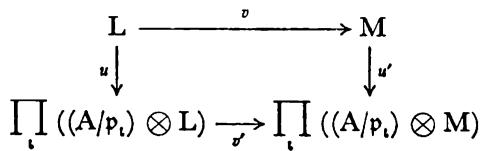
\includegraphics[keepaspectratio]{images/part001_964082be.jpg}}

其中 \(u\)（相应地 \(u'\)）是映射 \(x \mapsto (\phi_{\iota}(x))\)（相应地 \(y \mapsto (\psi_{\iota}(y)))\)），

\[
\phi_ {i} \colon \mathbf {L} \rightarrow (\mathbf {A} / \mathfrak {p} _ {i}) \otimes \mathbf {L}
\]

（相应地 \(\psi_{t}\colon\mathbf{M}\to(\mathbf{A}/p_{t})\otimes\mathbf{M}\)）是典范映射，而 \(v'\) 是诸 \(1_{\mathbf{A}/p_{t}}\otimes v\) 的乘积。于是 \((\mathbf{A}/p)/(m/p_{t})\otimes_{\mathbf{A}/p_{t}}((\mathbf{A}/p_{t})\otimes_{\mathbf{A}}\mathbf{M})=(\mathbf{A}/m)\otimes_{\mathbf{A}}\mathbf{M}\)，且由于 \(A/p_{t}\) 是局部整环，由论证的第一部分可得每个 \(1_{\mathbf{A}/p_{t}}\otimes v\) 都是同构；从而 \(v'\) 也是同构。另一方面，由于 A 是约化的，\(\bigcap_{i} p_{i} = (0)\)（\(\S 2\) 2 第 6 节命题 13），又因 L 是自由的，故 \(\bigcap_{i} (p_{i} L) = 0\)（《代数》第 II 章 \(\S 3\) 3 第 7 节注）；由于 \(p_{i} L\) 是 \(\phi_{i}\) 的核，这表明 \(u\) 是单射。由此推出 \(v' \circ u = u' \circ v\) 是单射，因而 \(v\) 是单射；而按定义 \(v\) 是满射，故这表明 M 是自由的。

\subsection{由局部到整体的过渡}

命题 8. 设 A 是一个环，m 是 A 的一个极大理想，M 是一个 A-模。若存在 A 的理想 a，使得 m 是 A 的包含 a 的唯一极大理想，且 aM = 0，则典范同态 \(M \rightarrow M_{m}\) 是双射。

此时 A/a 是以 m/a 为极大理想的局部环；可以把 M 视为一个 (A/a)-模；对一切 \(s \in A - m\)，s 在 A/a 中的典范像是可逆的，因而 M 的位似 \(x \mapsto sx\) 是双射，这源于把 \(M_{m}\) 定义为泛问题的解（§2 第 2 节）；由此即得命题。

特别地，若存在 \(k \geqslant 0\) 使 \(\mathfrak{m}^k\mathbf{M} = 0\)，则同态 \(\mathbf{M} \to \mathbf{M}_m\) 是双射（§1 第 1 节命题 1 的推论）。

命题 9. 设 A 是一个环，m 是 A 的一个极大理想，M 是一个 A-模，k 是一个整数 \(\geqslant0\)。典范同态 \(M\to M_{m}/m^{k}M_{m}\) 是满射，其核为 \(m^{k}M\)，并且给出 \(M/m^{k}M\) 到 \(M_{m}/m^{k}M_{m}\) 上的一个同构。

由于情形 \(k=0\) 是平凡的，设 \(k\geqslant1\)。由命题 8，典范同态 \(\mathbf{M}/\mathfrak{m}^{k}\mathbf{M}\to(\mathbf{M}/\mathfrak{m}^{k}\mathbf{M})_{\mathfrak{m}}\) 是双射。另一方面，\((\mathbf{M}/\mathfrak{m}^{k}\mathbf{M})_{\mathfrak{m}}\) 典范地等同于 \(\mathbf{M}_{\mathfrak{m}}/(\mathfrak{m}^{k}\mathbf{M})_{\mathfrak{m}}\)（§2 第 4 节定理 1），因而 \((\mathfrak{m}^{k}\mathbf{M})_{\mathfrak{m}}=\mathfrak{m}^{k}\mathbf{M}_{\mathfrak{m}}\)（§2 第 7 节命题 18 的推论），从而存在 \(\mathbf{M}/\mathfrak{m}^{k}\mathbf{M}\) 到 \(\mathbf{M}_{\mathfrak{m}}/\mathfrak{m}^{k}\mathbf{M}_{\mathfrak{m}}\) 上的一个同构，它把元素 \(x\in\mathbf{M}\) 的类映为 \(x/1\) 的类。

推论. 设 A 是一个环，\(m_{1}, m_{2}, \ldots, m_{n}\) 是 A 的互不相同的极大理想，M 是一个 A-模，\(k_{1}, k_{2}, \ldots, k_{n}\) 是整数 \(\geqslant 0\)。从 M 到 \(\prod_{i=1}^{n} \mathbf{M}_{\mathfrak{m}_{i}}/\mathfrak{m}_{i}^{k_{i}} \mathbf{M}_{\mathfrak{m}_{i}}\) 的典范同态是满射，其核为 \(\left(\bigcap_{i=1}^{n} \mathfrak{m}_{i}^{k_{i}}\right) \mathbf{M}\)。

这容易由命题 9 以及 §1 第 2 节命题 6 得出，因为诸 \(\mathfrak{m}_{i}^{k_{i}}\) 两两互素（§1 第 2 节命题 3）。

在本节余下部分，A 表示一个环，\(\Omega(A)\)（或 \(\Omega\)）表示 \(A\) 的极大理想的集合。

命题 10. A-模 \(\bigoplus_{m\in\Omega}A_m\)，即诸 \(A_m\)（其中 \(m\in\Omega\)）的直和，是忠实平坦的。

每个 \(A_{m}\) 都是平坦 A-模（\(\S\) 2 第 4 节定理 1），因而 \(E = \bigoplus_{m \in \Omega} A_{m}\) 是平坦的（第 I 章 \(\S\) 2 第 3 节命题 2）。此外，对 A 的每个极大理想 m，\(mA_{m}\) 是 \(A_{m}\) 的唯一极大理想，故 \(mA_{m} \neq A_{m}\)，由此推出 \(mE \neq E\)，从而 E 是忠实平坦的（第 I 章 \(\S\) 3 第 1 节命题 1 (d)）。

定理 1. 设 M、N 是两个 A-模，\(u: \mathbf{M} \to \mathbf{N}\) 是一个 A-同态，且对每个 \(m \in \Omega\)，设 \(u_m: \mathbf{M}_m \to \mathbf{N}_m\) 是相应的 \(\mathbf{A}_m\)-同态（§2 第 2 节注 5）。为使 \(u\) 是单射（相应地，满射、双射、零射），必须且只需对每个 \(m \in \Omega\)，\(u_m\) 是单射（相应地，满射、双射、零射）。

说对每个 \(m \in \Omega\) \(u_m\) 是单射（相应地，满射、双射、零射），等价于说同态 \(\bigoplus_{m} u_m: \bigoplus_{m} M_m \to \bigoplus_{m} N_m\) 具有同样的性质。但 \(\bigoplus_{m} M_m = M \otimes_A E\)，\(\bigoplus_{m} N_m = N \otimes_A E\)，且 \(\bigoplus_{m} u_m = u \otimes 1\)，其中 \(E = \bigoplus_{m} A_m\)；由于 \(E\) 是忠实平坦的（命题 10），定理由第 I 章 §3 第 1 节命题 1 (c) 及命题 2 得出。

推论 1. 设 M 是一个 A-模，N 是 M 的一个子模，x 是 M 的一个元素。为使 \(x \in N\)，必须且只需对每个 \(m \in \Omega\)，x 在 \(M_{m}\) 中的典范像属于 \(N_{m}\)。

设 \(\bar{x}\) 是 \(x\) 在 M/N 中的类；说 \(x \in N\)，意指从 A 到 M/N 的 A-线性映射 \(u: \alpha \mapsto \alpha \bar{x}\) 是零射。现在，\((\mathrm{M} / \mathrm{N})_{\mathfrak{m}}\) 等同于 \(\mathrm{M}_{\mathfrak{m}} / \mathrm{N}_{\mathfrak{m}}\)（§2 第 4 节定理 1），而 \(u_{\mathfrak{m}}: \mathrm{A}_{\mathfrak{m}} \to \mathrm{M}_{\mathfrak{m}} / \mathrm{N}_{\mathfrak{m}}\) 等同于映射 \(\lambda \mapsto \lambda \bar{x}_{\mathfrak{m}}\)，其中 \(\bar{x}_{\mathfrak{m}}\) 是模 \(\mathrm{N}_{\mathfrak{m}}\) 意义下的类，即 \(x\) 在 \(\mathrm{M}_{\mathfrak{m}}\) 中的典范像的类。由于由定理 1，关系 \(u = 0\) 等价于对一切 m 有 \(u_{\mathfrak{m}} = 0\)，这就证明了推论。

推论 2. 设 \(\mathbf{M}\) 是一个 A-模，且对每个 \(\mathfrak{m} \in \Omega\)，设 \(f_{\mathfrak{m}}\) 是典范映射 \(\mathbf{M} \to \mathbf{M}_{\mathfrak{m}}\)。同态 \(x \mapsto (f_{\mathfrak{m}}(x))\)（从 \(\mathbf{M}\) 到 \(\prod_{\mathfrak{m} \in \Omega} \mathbf{M}_{\mathfrak{m}}\)）是单射。

在 N = 0 的情形应用推论 1 可见，关系 x = 0 等价于 \(f_{m}(x) = 0\) 对一切 \(m \in \Omega\) 成立。

推论 3. (i) 设 \(\mathfrak{b}\) 是 \(\mathbf{A}\) 的一个理想，a 是 \(\mathbf{A}\) 的一个元素。为使 \(a \in \mathfrak{b}\)，必须且只需对每个 \(\mathfrak{m} \in \Omega\)，\(a\) 在 \(\mathbf{A}_{\mathfrak{m}}\) 中的典范像属于 \(\mathfrak{b}\mathbf{A}_{\mathfrak{m}}\)。

\begin{enumerate}
\def\labelenumi{(\roman{enumi})}
\setcounter{enumi}{1}
\tightlist
\item
  特别地，设 \(b\) 与 \(c\) 是 \(A\) 的两个元素。为使 \(c\) 是 \(b\) 的倍元，必须且只需对每个 \(m \in \Omega\)，\(c\) 在 \(A_m\) 中的典范像是 \(b\) 的典范像的倍元。
\end{enumerate}

由于 \(\mathfrak{bA}_{m} = \mathfrak{b}_{m}\)（§2 第 7 节命题 18 的推论），(i) 是推论 1 的特殊情形；(ii) 由把 (i) 应用于理想 Ab 而得。

推论 4. 设 A 是一个整环，K 是其分式域，M 是一个无挠 A-模，使得 M 典范地等同于 \(\mathbf{K} \otimes_{\mathbf{A}} \mathbf{M}\) 的一个 A-子模。那么，对每个 \(\mathfrak{m} \in \Omega\)，\(\mathbf{M}_{\mathfrak{m}}\) 典范地等同于 \(\mathbf{K} \otimes_{\mathbf{A}} \mathbf{M}\) 的一个 A-子模，且 \(\mathbf{M} = \bigcap_{\mathfrak{m} \in \Omega} \mathbf{M}_{\mathfrak{m}}\)。

由于 M 等同于 \(K \otimes_{A} M\) 的一个子模，故 \(M_{m}\) 等同于 \(A_{m}\)-模 \((\mathbf{K} \otimes_{\mathbf{A}} \mathbf{M})_{\mathfrak{m}} = \mathbf{K}_{\mathfrak{m}} \otimes_{\mathbf{A}} \mathbf{M}\) 的一个子模（§2 第 4 节定理 1）；由于 \(K_{m} = K\)，我们立即看出 \(M_{m}\) 是无挠的；此外，图的交换性

\[
\begin{array}{c} \mathbf {M} \longrightarrow \mathbf {K} \otimes_ {\mathbf {A}} \mathbf {M} \\ \Big \downarrow \qquad \qquad \qquad \qquad \qquad \qquad \qquad \qquad \Big \downarrow \\ \mathbf {M} _ {\mathfrak {m}} \longrightarrow (\mathbf {K} \otimes_ {\mathbf {A}} \mathbf {M}) _ {\mathfrak {m}} \end{array}
\]

证明典范映射 \(M \rightarrow M_{m}\) 是单射。于是该推论由把推论 1 应用于 A-模 \(K \otimes_{A} M\) 及其子模 M 而得。

特别地，对每个整环 A，

\[
\mathbf {A} = \bigcap_ {\mathfrak {m} \in \Omega} \mathbf {A} _ {\mathfrak {m}}.\tag{2}
\]

推论 5. 设 A 是一个环。A-模 \(\mathbf{A}^n\) 的每个由 \(n\) 个元素组成的生成系都是 \(\mathbf{A}^n\) 的一个基。

设 \((e_i)_{1\leqslant i\leqslant n}\) 是 \(\mathbf{A}^n\) 的典范基，\((x_i)_{1\leqslant i\leqslant n}\) 是 \(\mathbf{A}^n\) 的一个由 \(n\) 个元素组成的生成系，\(u\colon \mathbf{A}^n\to \mathbf{A}^n\) 是满足 \(u(e_i) = x_i\)（对 \(1\leqslant i\leqslant n\)）的 A-线性映射。由假设 \(u\) 是满射，需要证明 \(u\) 是单射。凭定理 1，这可以立即化为 \(\mathbf{A}\) 是局部环的情形；若 \(\mathfrak{m}\) 是 \(\mathbf{A}\) 的极大理想，则 \(1\otimes x_i\)（\(1\leqslant i\leqslant n\)）在 \((\mathrm{A / m})^n\) 中构成自由 \((\mathrm{A / m})\)-模 \((\mathrm{A / m})^n\) 的一个生成系；由于 \(\mathrm{A / m}\) 是域，该生成系是 \((\mathrm{A / m})^n\) 的一个基；由于 \(\mathbf{A}^n\) 是自由 A-模，我们由命题 5 推出 \((x_i)\) 是 \(\mathbf{A}^n\) 的一个基。

命题 11. 设 M 是一个 A-模，N 是一个有限生成 A-模，\(u: \mathbf{M} \to \mathbf{N}\) 是一个同态。为使 \(u\) 是满射，必须且只需对每个 \(\mathfrak{m} \in \Omega\)，同态 \(\mathbf{M} / \mathfrak{m}\mathbf{M} \to \mathbf{N} / \mathfrak{m}\mathbf{N}\)（由 \(u\) 取商而得）是满射。

由定理 1，为使 \(u\) 是满射，必须且只需 \(u_{\mathfrak{m}}: \mathrm{M}_{\mathfrak{m}} \to \mathrm{N}_{\mathfrak{m}}\) 对一切 \(\mathfrak{m} \in \Omega\) 是满射。由于 \(\mathrm{A}_{\mathfrak{m}}\) 是局部环且 \(\mathrm{N}_{\mathfrak{m}}\) 是有限生成 \(\mathrm{A}_{\mathfrak{m}}\)-模，这等价于说由取商得到的同态 \(u_{\mathfrak{m}}': \mathrm{M}_{\mathfrak{m}} / \mathrm{mM}_{\mathfrak{m}} \to \mathrm{N}_{\mathfrak{m}} / \mathrm{mN}_{\mathfrak{m}}\) 是满射（第 2 节命题 4 的推论 1）；而 \(\mathrm{M}_{\mathfrak{m}} / \mathrm{mM}_{\mathfrak{m}}\)（相应地 \(\mathrm{N}_{\mathfrak{m}} / \mathrm{mN}_{\mathfrak{m}}\)）等同于 \(\mathrm{M} / \mathrm{mM}\)（相应地 \(\mathrm{N} / \mathrm{mN}\)）（命题 9），由此即得命题。

命题 12. 设 E、F、G 是三个 A-模，\(v: \mathbf{G} \to \mathbf{F}\) 与 \(u: \mathbf{E} \to \mathbf{F}\) 是同态。假设 E 是有限表示的。为使存在同态 \(w: \mathbf{E} \to \mathbf{G}\) 使 \(u\) 分解为 \(\mathbf{E} \xrightarrow{w} \mathbf{G} \xrightarrow{v} \mathbf{F}\)，必须且只需对每个 \(m \in \Omega\)，存在同态 \(w^m: \mathbf{E}_m \to \mathbf{G}_m\) 使 \(u_m: \mathbf{E}_m \to \mathbf{F}_m\) 分解为 \(\mathbf{E}_m \xrightarrow{w^m} \mathbf{G}_m \xrightarrow{v_m} \mathbf{F}_m\)。

存在满足上述命题的 w 等价于下面的性质：u 属于映射

\[
r = \operatorname{Hom} (1 _ {\mathbf {E}}, v): \operatorname{Hom} _ {\mathbf {A}} (\mathbf {E}, \mathbf {G}) \rightarrow \operatorname{Hom} _ {\mathbf {A}} (\mathbf {E}, \mathbf {F}).
\]

现在，\((\mathrm{Hom}_{\mathbf{A}}(\mathrm{E},\mathbf{F}))_{\mathfrak{m}}\)（相应地 \((\mathrm{Hom}_{\mathbf{A}}(\mathrm{E},\mathbf{G}))_{\mathfrak{m}}\)）典范地等同于 \(\mathrm{Hom}_{\mathbf{A}_{\mathfrak{m}}}(\mathrm{E}_{\mathfrak{m}},\mathrm{F}_{\mathfrak{m}})\)（相应地 \(\mathrm{Hom}_{\mathbf{A}_{\mathfrak{m}}}(\mathrm{E}_{\mathfrak{m}},\mathrm{G}_{\mathfrak{m}})\)）（§2 第 7 节命题 19 (i)），u 在 \((\mathrm{Hom}_{\mathbf{A}}(\mathrm{E},\mathbf{F}))_{\mathfrak{m}}\) 中的典范像等同于 \(u_{m}\)，\(r_{m}\) 等同于 \(\mathrm{Hom}_{\mathbf{A}_{\mathfrak{m}}}(1_{\mathbf{E}_{\mathfrak{m}}},v_{\mathfrak{m}})\)，而 \(P_{m}\) 等同于 \(r_{m}\) 的像。于是该命题由把定理 1 的推论 1 应用于 \(\mathrm{Hom}_{\mathbf{A}}(\mathrm{E},\mathbf{F})\) 及其子模 P 而得。

推论 1. 设 M 是一个 A-模，N 是 M 的一个子模，使得 M/N 是有限表示的。为使 N 是 M 的一个直因子，必须且只需对每个 \(m \in \Omega\)，\(N_{m}\) 是 \(M_{m}\) 的一个直因子。

说 N 是 M 的直因子，意指 M/N 上的恒同同态分解为 \(M/N \xrightarrow{w} M \xrightarrow{\phi} M/N\)，其中 \(\phi\) 是典范同态，w 是一个同态（《代数》第 II 章 §1 第 9 节命题 14）；由于 \((\mathrm{M}/\mathrm{N})_{\mathrm{m}} = \mathrm{M}_{\mathrm{m}}/\mathrm{N}_{\mathrm{m}}\) 且 \(\phi_{m}\) 是典范同态 \(M_{m} \to M_{m}/N_{m}\)，故由命题 12 容易得出推论。

推论 2. 设 M 是一个有限生成的自由 A-模，N 是 M 的一个子模且是有限生成的自由 A-模。为使 N 是 M 的一个直因子，必须且只需对所有 m ∈ Ω，mN = N ∩ (mM)。

按定义 M/N 是有限表示的；另一方面，\(N_{m}\) 与 \(M_{m}\) 是有限生成的自由 \(A_{m}\)-模。为使 \(N_{m}\) 是 \(M_{m}\) 的一个直因子，必须且只需典范映射 \(N_{m}/mN_{m} \rightarrow M_{m}/mM_{m}\) 是单射（第 2 节命题 6）；这等价于说典范映射 \(N/mN \rightarrow M/mM\) 是单射（命题 9），而由于其核为 \((N \cap mM)/mN\)，这就证明了推论。

命题 12（相应地，其推论 1）尤其将应用于 A 是 Noether 环且 E（相应地，M/N）是有限生成 A-模的情形（第 I 章 §2 第 8 节引理 8）。

\subsection{平坦性的局部化}

命题 13. 设 S 是环 A 的一个乘性子集，M 是一个 A-模。若 M 是平坦的（相应地，忠实平坦的），则 \(S^{-1}M\) 是平坦（相应地，忠实平坦）\(S^{-1}A\)-模，并且是平坦 A-模。

由于 \(S^{-1}M = M \otimes_{A} S^{-1}A\)，第一个断言由第 I 章 §2 第 7 节命题 8 的推论 2（相应地，第 I 章 §3 第 3 节命题 5）得出；此外，\(S^{-1}A\) 是平坦 A-模（§2 第 4 节定理 1）；因此若 M 是平坦 A-模，则凭第 I 章 §2 第 7 节命题 8 的推论 3，\(S^{-1}M\) 也是。

注. 若 N 是一个 \(S^{-1}A\)-模，则 \(S^{-1}N\) 等同于 N，因而这等价于说 N 是平坦 \(S^{-1}A\)-模或平坦 A-模。

命题 14. 设 A 是一个环，B 是一个交换 A-代数，T 是 B 的一个乘性子集。若 N 是一个作为 A-模时平坦的 B-模，则 \(T^{-1}N\) 是平坦 A-模。

\(T^{-1}N = T^{-1}B \otimes_{B} N\)；于是该命题由第 I 章 §2 第 7 节命题 8 得出，其中 A 换成 B，B 换成 A，E 换成 \(T^{-1}B\)，F 换成 N。

命题 15. 设 A、B 是两个环，\(\phi: A \to B\) 是一个同态，N 是一个 B-模。下列性质等价：

\begin{enumerate}
\def\labelenumi{(\alph{enumi})}
\item
  N 是平坦 A-模。
\item
  对每个 \(\mathfrak{n}\)（即 \(\mathbf{B}\) 的极大理想），\(\mathbf{N}_{\mathfrak{n}}\) 是平坦 A-模。
\item
  对每个 \(\mathfrak{n}\)（即 \(\mathbf{B}\) 的极大理想），若记 \(\mathfrak{m} = \bar{\phi}^{-1}(\mathfrak{n})\)，则 \(\mathbf{N}_{\mathfrak{n}}\) 是平坦 \(\mathbf{A}_{\mathfrak{m}}\)-模。
\end{enumerate}

对所有 \(a \notin m\)，由 a 诱导的 \(N_{n}\) 的位似是双射，故 \(N_{n}\) 典范地等同于 \((\mathrm{N}_{\mathrm{n}})_{\mathrm{m}}\)，于是 (b) 与 (c) 的等价性由

命题 13 后面的注得出；(a) 蕴含 (b) 这一事实是命题 14 的特殊情形。剩下的要证明 (b) 蕴含 (a)，即若 (b) 成立，则对每个单的 A-模同态 \(u: \mathbf{M} \to \mathbf{M}'\)，同态 \(v = 1 \otimes u: \mathbf{N} \otimes_{\mathbf{A}} \mathbf{M} \to \mathbf{N} \otimes_{\mathbf{A}} \mathbf{M}'\) 是单射。现在，\(v\) 也是 B-模同态，而为使它是单射，必须且只需 \(v_n: (\mathbf{N} \otimes_{\mathbf{A}} \mathbf{M})_n \to (\mathbf{N} \otimes_{\mathbf{A}} \mathbf{M}')_n\) 对每个 \(n\)（即 \(B\) 的极大理想）都是单射（第 3 节定理 1）。由于

\[
(\mathbf {N} \otimes_ {\mathbf {A}} \mathbf {M}) _ {n} = \mathbf {B} _ {n} \otimes_ {\mathbf {B}} (\mathbf {N} \otimes_ {\mathbf {A}} \mathbf {M}) = \mathbf {N} _ {n} \otimes_ {\mathbf {A}} \mathbf {M},
\]

\(v_{n}\) 正是同态 \(1 \otimes u: N_{n} \otimes_{A} M \to N_{n} \otimes_{A} M'\)，由于按假设 \(N_{n}\) 是平坦 A-模，它是单射的。

推论. 为使一个 A-模 M 是平坦的（相应地，忠实平坦的），必须且只需对 A 的每个极大理想 m，\(M_{m}\) 是平坦（相应地，忠实平坦）\(A_{m}\)-模。

条件的必要性由命题 13 得出。反之，若对 A 的每个极大理想 m，\(M_{m}\) 是平坦 \(A_{m}\)-模，则凭命题 15 应用于 \(\phi\) 是恒同的情形，M 是平坦 A-模。最后，若对一切 m，\(M_{m}\) 是忠实平坦 \(A_{m}\)-模，则 \(mM_{m} = mA_{m}M_{m} \neq M_{m}\)，从而对一切 m 有 \(mM \neq M\)（第 3 节命题 9），这就证明 M 是忠实平坦 A-模（第 I 章 §3 第 1 节命题 1 (d)）。

\subsection{半局部环}

命题 16. 设 A 是一个环。下列性质等价：

\begin{enumerate}
\def\labelenumi{(\alph{enumi})}
\item
  \(\mathbf{A}\) 的极大理想集合是有限的；
\item
  A 对其 Jacobson 根的商是有限个域的直合成。
\end{enumerate}

设 A 对其 Jacobson 根 \(\Re\) 的商是有限个域的直合成。那么 \(\Re\) 只有有限多个理想，\(a\ fortiori\) 只有有限多个极大理想。由于每个极大理想都包含 \(\Re\)（《代数》第 VIII 章 §6 第 2 节定义 2），A 的极大理想是 \(\Re\) 的极大理想在典范同态 A \(\rightarrow\) \(\Re\) 下的原像；因而它们个数有限。

反之，设 A 只有有限多个互不相同的极大理想 \(m_{1}, \ldots, m_{n}\)。诸 \(A/m_{i}\) 是域，且由 §1 第 2 节命题 5，典范映射 \(A \to \prod_{i=1}^{n} A/m_{i}\) 是满射；由于其核 \(\bigcap_{i=1}^{n} m_{i}\) 是 Jacobson 根 R（《代数》第 VIII 章 §6 第 2 节定义 2），A/R 同构于 \(\prod_{i=1}^{n} A/m_{i}\)。

定义 4. 若一个环满足命题 16 的等价条件 (a)、(b)，则称它为半局部环。

例. 每个局部环都是半局部的。半局部环的每个商环都是半局部的。半局部环的每个有限乘积都是半局部的。

* 若 A 是一个 Noether 半局部环，B 是一个作为 A-模为有限生成的 A-代数，则 B 是半局部的（第 IV 章 §2 第 5 节命题 9 的推论 3）。*

下述命题给出另一个例子，它推广了局部环 \(A_{p}\) 的构造：

命题 17. 设 A 是一个环，\(p_1, \ldots, p_n\) 是 A 的素理想。记 \(S = \bigcap_{i=1}^{n} (A - p_i) = A - \bigcup_{i=1}^{n} p_i\)。

\begin{enumerate}
\def\labelenumi{(\alph{enumi})}
\item
  环 \(\mathbf{S}^{-1}\mathbf{A}\) 是半局部的；若 \(\mathfrak{q}_1, \ldots, \mathfrak{q}_r\) 是诸 \(\mathfrak{p}_i\) 之中（按包含关系）互不相同的极大元，则 \(\mathbf{S}^{-1}\mathbf{A}\) 的极大理想是诸 \(\mathbf{S}^{-1}\mathfrak{q}_j\)（\(1 \leqslant j \leqslant r\)），且这些理想互不相同。
\item
  环 \(\mathbf{A}_{\mathfrak{p}_i}\) 典范同构于 \((\mathbf{S}^{-1}\mathbf{A})_{\mathbf{S}^{-1}\mathfrak{p}_i}\)（对 \(1 \leqslant i \leqslant n\)）。
\item
  若 \(\mathbf{A}\) 是一个整环，则 \(\mathbf{S}^{-1}\mathbf{A} = \bigcap_{i=1}^{n}\mathbf{A}_{p_i}\)（在 \(\mathbf{A}\) 的分式域中）。
\end{enumerate}

(a) A 的与 S 不相交的理想是含于诸 \(p_{i}\) 之并从而含于至少一个 \(p_{i}\) 之中的理想（§1 第 1 节命题 2）；因此诸 \(q_{j}\) 是与 S 不相交的理想集合的极大元；于是由 §2 第 5 节命题 11 (ii)，诸 \(S^{-1}q_{j}\) 是 \(S^{-1}A\) 的极大理想。

(b) 是 §2 第 5 节命题 11 (iii) 的特殊情形。

(c) 设 A 是一个整环。若 \(p_{i} \subset p_{k}\)，则 \(A_{p_{i}} \supset A_{p_{k}}\)；因此为证 (c)，可以设诸 \(p_{i}\) 两两不可比较。于是由 (a) 及第 3 节定理 1 的推论 4 得 \(S^{-1}A = \bigcap_{i=1}^{n} (S^{-1}A)_{S^{-1}p_{i}}\)；再凭 (b) 即得 (c)。

若 A 是整环，则 \(S^{-1}A\) 也是整环，于是命题 17 给出了一个不是局部环的直合成的半局部环的例子（参见~第 III 章 §2 第 13 节）。

推论. 设 A 是一个整环，\(p_{1}, \ldots, p_{n}\) 是 A 的素理想，其中任意两个按包含关系都不可比较。若在 A 的分式域中 \(A = \bigcap_{i=1}^{n} A_{p_{i}}\)，则 A 的极大理想是 \(p_{1}, \ldots, p_{n}\)。

取 \(S = \bigcap_{i=1}^{n} (A - p_i), S^{-1} A = A\)（由命题 17 (c)）；于是 \(S\) 的元素在 \(A\) 中可逆，且 \(S^{-1} p_i = p_i\) 对一切 \(i\) 成立。我们的断言随即凭命题 17 (a) 得出。

\section{环的谱与模的支撑集}

\subsection{不可约空间}

定义 1. 若拓扑空间 X 的非空开集的每个有限交都非空，则称 X 为不可约的。

考虑 X 的开集的空族即可看出，不可约空间是非空的；为使拓扑空间 X 不可约，必须且只需它是非空的，且 X 的两个非空开集的交总是非空的（或者等价地说，两个异于 X 的闭集的并总是异于 X 的）。

命题 1. 设 X 是一个非空拓扑空间。下列条件等价：

\begin{enumerate}
\def\labelenumi{(\alph{enumi})}
\item
  \(\mathbf{X}\) 是不可约的；
\item
  \(\mathbf{X}\) 的每个非空开集在 \(\mathbf{X}\) 中稠密；
\item
  \(\mathbf{X}\) 的每个开集都是连通的。
\end{enumerate}

按定义，在 X 中稠密的集合是与每个非空开集都相交的集合，因此 (a) 与 (b) 等价。立刻可见 (c) 蕴含 (a)，因为若 \(U_{1}\) 与 \(U_{2}\) 是互不相交的非空开集，则 \(U_{1} \cup U_{2}\) 是一个不连通的开集。最后证明 (a) 蕴含 (c)：若 U 是一个不连通的开集，则它是两个互不相交的非空集合 \(U'\)、\(U''\) 的并，这两个集合在 U 中开，从而在 X 中也开，这蕴含 X 不是不可约的。

一个 Hausdorff 空间仅当它由单个点组成时才可能是不可约的。

拓扑空间 X 的子集 E 称为不可约集，如果 X 的子空间 E 是不可约的。为此，必须且只需对每对在 X 中开且与 E 相交的集合 U、V，\(U \cap V\) 也与 E 相交，或者（等价地）对每对在 X 中闭且满足 \(E \subset F \cup G\) 的集合 F、G，有 \(E \subset F\) 或 \(E \subset G\)。对 n 用归纳法，我们推出：若 \((\mathbf{F}_{i})_{1 \leq i \leq n}\) 是 X 的闭集的有限族且满足 \(E \subset \bigcup_{i=1}^{n} F_{i}\)，则存在指标 i 使 \(E \subset F_{i}\)。

命题 2. 在拓扑空间 X 中，为使一个集合 E 不可约，必须且只需其闭包 \(\overline{E}\) 不可约。

为使 X 的一个开集与 E 相交，必须且只需它与 \(\overline{E}\) 相交；于是命题由上面的注得出。

命题 3. (i) 若 X 是不可约空间，则 X 的每个非空开子集都不可约。

\begin{enumerate}
\def\labelenumi{(\roman{enumi})}
\setcounter{enumi}{1}
\item
  设 \((\mathbf{U}_{\alpha})_{\alpha \in \mathbf{A}}\) 是拓扑空间 \(\mathbf{X}\) 的一个由开集组成的非空覆盖，使得 \(\mathbf{U}_{\alpha} \cap \mathbf{U}_{\beta} \neq \varnothing\) 对每对指标 \((\alpha, \beta)\) 都成立。若诸集合 \(\mathbf{U}_{\alpha}\) 不可约，则空间 \(\mathbf{X}\) 不可约。
\end{enumerate}

(i) 若 \(\mathbf{X}\) 不可约，\(\mathbf{U} \subset \mathbf{X}\) 在 \(\mathbf{X}\) 中非空且开，\(\mathbf{V} \subset \mathbf{U}\) 在 \(\mathbf{U}\) 中非空且开，则 \(\mathbf{V}\) 也在 \(\mathbf{X}\) 中开，从而在 \(\mathbf{X}\) 中稠密，更加在 \(\mathbf{U}\) 中稠密。于是 \(\mathbf{U}\) 不可约（命题 1）。

(ii) 我们证明，对 X 中每个非空开集 V，\(V \cap U_{\alpha} \neq \varnothing\) 对一切 \(\alpha \in A\) 成立：由此按假设 \(V \cap U_{\alpha}\) 在 \(U_{\alpha}\) 中稠密，从而 V 在 X 中稠密，这证明 X 不可约（命题 1）。现在至少存在一个指标 \(\gamma\) 使 \(V \cap U_{\gamma} \neq \varnothing\)；由于 \(U_{\alpha} \cap U_{\gamma} \neq \varnothing\) 对一切 \(\alpha\) 成立，且 \(V \cap U_{\gamma}\) 在 \(U_{\gamma}\) 中稠密，故 \(U_{\alpha} \cap U_{\gamma} \cap V \neq \varnothing\)，更加有 \(U_{\alpha} \cap V \neq \varnothing\)，这就完成了 (ii) 的证明。

命题 4. 设 X 与 Y 是两个拓扑空间，f 是从 X 到 Y 的一个连续映射。对 X 的每个不可约子集 E，\(f(E)\) 是 Y 的一个不可约子集。

若 U、V 是 Y 的两个与 \(f(\mathrm{E})\) 相交的开集，则 \(\overline{f}^{-1}(\mathrm{U})\) 与 \(\overline{f}^{-1}(\mathrm{V})\) 是 X 的与 E 相交的开集。因此 \(\overline{f}^{-1}(\mathrm{U}) \cap \overline{f}^{-1}(\mathrm{V}) = \overline{f}^{-1}(\mathrm{U} \cap \mathrm{V})\) 与 E 相交，这蕴含 \(U \cap V\) 与 \(f(\mathrm{E})\) 相交，从而证明了命题。

定义 2. 拓扑空间 X 的每个极大不可约子集称为 X 的一个不可约分支。

由命题 2，\(\mathbf{X}\) 的每个不可约分支在 \(\mathbf{X}\) 中是闭的。

命题 5. 设 X 是一个拓扑空间。X 的每个不可约子集都含于 X 的一个不可约分支中，且 X 是其诸不可约分支的并。

为证第一个断言，凭 Zorn 引理，只需证明 \(\Im\)（即 \(X\) 的不可约子集之集）是归纳的。设 \(\mathfrak{G}\) 是 \(\Im\) 的一个按包含关系全序的子集；我们证明 \(E\)（诸集合 \(F \in \mathfrak{G}\) 的并）不可约。设 \(U\)、\(V\) 是 \(X\) 的两个与 \(E\) 相交的开集；由于 \(\mathfrak{G}\) 是全序的，存在与 U 和 V 都相交的集合 \(F \in \mathfrak{G}\)；由于 F 不可约，\(U \cap V\) 与 F 相交，从而也与 E 相交，这证明 E 不可约，从而 \(\mathfrak{G}\) 是归纳的。第二个断言由第一个得出，因为 X 的每个由单个点组成的子集都不可约。

推论. 拓扑空间 X 的每个连通分支都是 X 的若干不可约分支的并。

由命题 1，X 的每个不可约子空间都连通，从而含于 X 的一个连通分支中。

注意，X 的两个不同的不可约分支可能有公共点（习题 11）。

命题 6. 设 X 是一个拓扑空间，\((\mathrm{P}_{i})_{1\leq i\leq n}\) 是 X 的一个由不可约闭集组成的有限覆盖。则 X 的不可约分支是诸 \(P_{i}\) 的集合的（按包含关系的）极大元。

我们可以限于诸 \(P_{i}\) 两两不可比较的情形。若 E 是 X 的一个不可约子集，则 \(E \subset \bigcup_{i=1}^{n} P_{i}\)，从而 E 含于某个闭集 \(P_{i}\) 之中；这证明诸 \(P_{i}\) 是 X 仅有的极大不可约子集。

推论. 设 X 是一个拓扑空间，E 是一个只有有限多个不同不可约分支 \(Q_{i}\)（\(1 \leqslant i \leqslant n\)）的子空间；则 X 中闭包 \(\overline{E}\) 的不可约分支是诸 \(\overline{Q}_{i}\)（即 \(Q_{i}\) 的闭包，\(1 \leqslant i \leqslant n\)），且 \(\overline{Q}_{i} \neq \overline{Q}_{j}\) 对 \(i \neq j\) 成立。

\(\overline{\mathbf{E}}\) 是诸 \(\overline{\mathbf{Q}}_i\) 的并，它们不可约（命题 2）；由于 \(\mathbf{Q}_i\) 在 \(\mathbf{E}\) 中闭，故 \(\overline{\mathbf{Q}}_i \cap \mathbf{E} = \mathbf{Q}_i\)；由于 \(\mathbf{Q}_i \not\subset \mathbf{Q}_j\) 对 \(i \neq j\) 成立，故 \(\overline{\mathbf{Q}}_i \not\subset \overline{\mathbf{Q}}_j\)，从而凭命题 6 得该推论。

注. 设 X 只有有限多个不同的不可约分支 \(X_{i}\)（\(1 \leqslant i \leqslant n\)）；则 \(U_{i} = \complement\left(\bigcup_{j \neq i} X_{j}\right)\) 在 X 中开且在 \(X_{i}\) 中稠密，因为 \(X_{i} \not\subset \bigcup_{j \neq i} X_{j}\)；于是诸 \(U_{i}\)（\(1 \leqslant i \leqslant n\)）是 X 的非空开集，它们不可约（命题 2）、两两不相交，且它们的并在 X 中稠密。

命题 7. 设 U 是拓扑空间 X 的一个开子集。映射 \(V \mapsto \overline{V}\)（闭包取在 X 中）是从 U 的在 U 中闭的不可约子集之集到 X 的在 X 中闭且与 U 相交的不可约子集之集上的双射；逆双射是 \(Z \mapsto Z \cap U\)。特别地，此双射把 U 的不可约分支之集映到 X 的与 U 相交的不可约分支之集上。

若 V 在 U 中闭且不可约，则 \(\overline{V}\) 不可约（命题 2）且 \(V = \overline{V} \cap U\)。反之，若 Z 不可约、在 X 中闭且与 U 相交，则 \(Z \cap U\) 是 Z 的非空开子集，从而不可约（命题 3）且在 Z 中稠密；由于 Z 是闭的，\(Z = \overline{Z \cap U}\)。这就证明了命题。

\subsection{Noether 拓扑空间}

定义 3. 若拓扑空间 X 的闭子集的每个非空集合（按包含关系排序）都有极小元，则称 X 为 Noether 空间。

这等价于说 X 的开子集的每个非空集合（按包含关系排序）都有极大元，或说闭（相应地，开）集的每个递减（相应地，递增）序列都是平稳的（《集合论》第 III 章 §6 第 5 节命题 6）。

命题 8. (i) Noether 空间的每个子空间都是 Noether 的。

\begin{enumerate}
\def\labelenumi{(\roman{enumi})}
\setcounter{enumi}{1}
\item
  设 \((\mathbf{A}_i)_{i\in I}\) 是拓扑空间 \(\mathbf{X}\) 的一个有限覆盖。若 \(\mathbf{A}_i\)（\(\mathbf{X}\) 的子空间）都是 Noether 的，则 \(\mathbf{X}\) 是 Noether 的。

\end{enumerate}

(i) 设 X 是一个 Noether 空间，A 是 X 的一个子空间，\((\mathbf{F}_{n})\) 是 A 的在 A 中闭的子集的一个递减序列；则 \(F_{n} = \overline{F}_{n} \cap A\)，且 \(\overline{F}_{n}\)（诸 \(F_{n}\) 在 X 中的闭包）构成 X 的闭子集的一个递减序列。由于该序列是平稳的，故序列 \((\mathbf{F}_{n})\) 也是平稳的。

(ii) 设 \((\mathbf{G}_n)_{n\geqslant 0}\) 是 \(\mathbf{X}\) 的闭子集的一个递减序列；按假设，序列 \((\mathrm{G}_n\cap \mathrm{A}_i)_{n\geqslant 0}\) 都是平稳的。由于 I 有限，存在整数 \(n_0\)，使得对 \(n\geqslant n_0\)，\(\mathbf{G}_n\cap \mathbf{A}_i = \mathbf{G}_{n_0}\cap \mathbf{A}_i\) 对一切 \(i\in \mathbf{I}\) 成立。但

\[
\mathbf {G} _ {n} = \bigcup_ {i \in I} \left(\mathbf {G} _ {n} \cap \mathbf {A} _ {i}\right)
\]

因而序列 \((\mathbf{G}_n)\) 是平稳的，且 \(\mathbf{X}\) 是 Noether 的。

命题 9. 为使拓扑空间 X 是 Noether 的，必须且只需 X 的每个开集都是拟紧的。

为证该条件是必要的，凭命题 8，只需证明每个 Noether 空间 X 都是拟紧的。设 \((\mathbf{U}_{\iota})_{\iota\in\mathbf{I}}\) 是 X 的一个开覆盖；诸 \(U_{\iota}\) 的有限并组成的集合非空，从而有极大元 \(V=\bigcup_{\iota\in H}U_{\iota}\)，其中 H 是 I 的有限子集。按定义，\(V\cup U_{\iota}=V\) 对一切 \(\iota\in I\) 成立，因而 V=X。

反之，设 X 的每个开集都是拟紧的，并设 \((\mathbf{U}_{n})\) 是 X 的开子集的一个递增序列。诸 \(U_{n}\) 的并 V 是开的从而拟紧；由于 \((\mathbf{U}_{n})\) 是 V 的开覆盖，\((\mathbf{U}_{n})\) 有一个有限子族覆盖 V，因而对某个指标 n 有 \(V = U_{n}\)，这证明序列 \((\mathbf{U}_{n})\) 是平稳的。

引理 1（``Noether 归纳法原理''）. 设 E 是一个每个非空子集都有极小元的有序集。设 F 是 E 的具有下述性质的子集：若 \(a \in E\) 使得关系 \(x < a\) 蕴含 \(x \in F\)，则 \(a \in F\)。那么 \(F = E\)。

设 \(\mathbf{F} \neq \mathbf{E}\)；那么 \(\complement\mathbf{F}\) 将有极小元 \(b\)。按定义，\(x \in \mathbf{F}\) 对一切 \(x < b\) 成立，这蕴含 \(b \in \mathbf{F}\)，矛盾。

命题 10. 若 X 是一个 Noether 空间，则 X 的不可约分支之集（更加，X 的连通分支之集）是有限的。

只需证明 X 是不可约闭子集的有限并（第 1 节命题 6）。我们证明 Noether 归纳法原理可以应用：取 E 为 X 的闭子集之集（按包含关系排序），F 为不可约闭子集的有限并组成的集。设 Y 是 X 的一个闭子集，使得 Y 的每个满足 \(\neq Y\) 的闭子集都属于 F。若 Y 不可约，则按定义 \(Y \in F\)；否则，Y 是两个异于 Y 的闭子集 \(Y_{1}, Y_{2}\) 的并。于是按假设 \(Y_{1} \in F\) 且 \(Y_{2} \in F\)，从而按 F 的定义 \(Y \in F\)。

特别地，由此得出一个 Hausdorff 的 Noether 空间必然是有限的。

\subsection{环的素谱}

设 A 是一个环，X 是 A 的素理想之集。对 A 的每个子集 M，我们用 V(M) 表示包含 M 的 A 的素理想之集；显然，若 a 是 M 生成的 A 的理想，则 V(M) = V(a)；若 M 由单个元素 f 组成，则我们用 V(f) 代替 V(\{f\})，且有 V(f) = V(Af)。映射 M \(\mapsto\) V(M) 关于 A 与 X 中的包含关系是递减的。此外，下列公式成立：

\begin{enumerate}
\def\labelenumi{(\arabic{enumi})}
\tightlist
\item
\end{enumerate}

\[
\mathbf {V} (0) = \mathbf {X}, \quad \mathbf {V} (1) = \varnothing ;\tag{1}
\]

\[
\mathrm{V} \left(\bigcup_ {i \in I} \mathrm{M} _ {i}\right) = \mathrm{V} \left(\sum_ {i \in I} \mathrm{M} _ {i}\right) = \bigcap_ {i \in I} \mathrm{V} (\mathrm{M} _ {i})\tag{2}
\]

对 A 的子集的每个族 \((\mathbf{M}_i)_{i\in I}\) 成立；

\[
\mathbf {V} (\mathfrak {a} \cap \mathfrak {a} ^ {\prime}) = \mathbf {V} (\mathfrak {a a} ^ {\prime}) = \mathbf {V} (\mathfrak {a}) \cup \mathbf {V} (\mathfrak {a} ^ {\prime})\tag{3}
\]

对 A 中理想的每个对 \(\mathfrak{a},\mathfrak{a}'\)。公式 (1) 与 (2) 是显然的；另一方面，公式 (3) 表示：为使 A 的素理想 \(\mathfrak{p}\) 包含理想 \(\mathfrak{a}\) 与 \(\mathfrak{a}'\) 之一，必须且只需它包含 \(\mathfrak{a}\mathfrak{a}'\) 或包含 \(\mathfrak{a} \cap \mathfrak{a}'\)；于是它是 §1 第 1 节命题 1 的推论。(1) 中第二个公式有下述逆命题：若 \(\mathfrak{a}\) 是 \(\mathbf{A}\) 的一个理想，使 \(V(\mathfrak{a}) = \varnothing\)，则 \(\mathfrak{a} = \mathbf{A}\)，因为不存在 \(\mathbf{A}\) 的包含 \(\mathfrak{a}\) 的极大理想。最后，若 \(\mathfrak{a}\) 是 \(\mathbf{A}\) 的一个理想，而 \(r(\mathfrak{a})\) 是它的根（§2 第 6 节定义 4），则

\[
\mathbf {V} (\mathfrak {a}) = \mathbf {V} (\mathfrak {r} (\mathfrak {a}))\tag{4}
\]

这由 §2 第 6 节命题 13 的推论 1 得出。

公式 (1) 至 (3) 表明，X 的子集 V(M) 满足一个拓扑的闭集公理（《一般拓扑学》第 I 章 §1 第 4 节）。

定义 4. 设 A 是一个环。A 的素理想之集 X，带上以诸 V(M)（M 跑遍 P(A)）为闭集的拓扑，称为 A 的素谱，记作 Spec(A)。这样定义的拓扑称为 X 上的谱拓扑或 Zariski 拓扑。

显然，关系 \(\operatorname{Spec}(\mathbf{A}) = \varnothing\) 等价于 \(\mathbf{A} = \{0\}\)。

设 X 是环 A 的素谱；对每个 \(f \in A\)，用 \(X_{f}\) 表示不包含 f 的 A 的素理想之集；则 \(\mathbf{X}_{f} = \mathbf{X} - \mathbf{V}(f)\)，因而 \(X_{f}\) 是开集。由 (2)，X 的每个闭子集都是形如 \(\mathrm{V}(f)\) 的闭集之交，故诸 \(X_{f}\) 构成 X 上谱拓扑的一个基。此外，由定义立即得出

\[
\mathbf {X} _ {0} = \varnothing , \quad \mathbf {X} _ {1} = \mathbf {X},\tag{5}
\]

更一般地，对 A 的每个可逆元 f 有 \(X_{f} = X\)；

\[
\mathrm{X} _ {f g} = \mathrm{X} _ {f} \cap \mathrm{X} _ {g} \quad \text {   for   all   } f, g \text {   in   A.   }\tag{6}
\]

对 X 的每个子集 Y，用 \(\Im(Y)\) 表示属于 Y 的 A 的素理想之交。显然 \(\Im(Y)\) 是 A 的理想，且映射 \(Y \mapsto \Im(Y)\) 关于 X 与 A 中的包含关系是递减的。显然，关系

\begin{enumerate}
\def\labelenumi{(\arabic{enumi})}
\setcounter{enumi}{6}
\tightlist
\item
\end{enumerate}

\[
\Im (\varnothing) = \mathbf {A}\tag{7}
\]

\[
\Im \left(\bigcup_ {\lambda \in L} Y _ {\lambda}\right) = \bigcap_ {\lambda \in L} \Im (Y _ {\lambda})\tag{8}
\]

对族 \((\mathbf{Y}_{\lambda})_{\lambda \in \mathbf{L}}\)（\(\mathbf{X}\) 的子集组成的族）成立。此外：

命题 11. 设 A 是一个环，a 是 A 的一个理想，Y 是 X = Spec(A) 的一个子集。

\begin{enumerate}
\def\labelenumi{(\roman{enumi})}
\item
  \(\mathbf{V}(\mathfrak{a})\) 在 \(\mathbf{X}\) 中闭，而 \(\Im (\mathbf{Y})\) 是 A 的一个等于其根的理想。
\item
  \(\Im(\mathrm{V}(\mathfrak{a}))\) 是 \(\mathfrak{a}\) 的根，且 \(\mathrm{V}(\Im(\mathrm{Y}))\) 是 \(\mathrm{Y}\) 在 \(\mathrm{X}\) 中的闭包。
\item
  映射 \(\Im\) 与 \(\mathbf{V}\) 定义互逆的两个递减双射，它们建立于 \(\mathbf{X}\) 的闭子集之集与 \(\mathbf{A}\) 的等于其根的理想之集之间。
\end{enumerate}

断言 (i) 与 (ii) 的第一个断言由定义及 §2 第 6 节命题 13 的推论 1 得出。若闭集 V(M)（对某个 M ⊂ A）包含 Y，则对每个素理想 p ∈ Y 有 M ⊂ p，从而 M ⊂ \(\mathfrak{I}\)(Y)，因而 V(M) ⊃ V(\(\mathfrak{I}\)(Y))；由于 Y ⊂ V(\(\mathfrak{I}\)(Y))，V(\(\mathfrak{I}\)(Y)) 是 X 中包含 Y 的最小闭集，这就完成了 (ii) 的证明。最后，由 (ii) 得出：若 a 是等于其根的一个理想，则 \(\mathfrak{I}\)(V(a)) = a；若 Y 在 X 中闭，则 V(\(\mathfrak{I}\)(Y)) = Y。这就证明了 (iii)。

由命题 11 立即得出：若 M 是 A 的任意子集而 Y 是 X 的任意子集，则 V(M) = V(\(\Im(V(M))\)) 且 \(\Im(Y) = \Im(V(\Im(Y)))\)。

推论 1. 对每个族 \((\mathbf{Y}_{\lambda})_{\lambda \in L}\)（由 \(\mathbf{X}\) 的闭子集组成），\(\Im\left(\bigcap_{\lambda \in L} \mathbf{Y}_{\lambda}\right)\) 是诸理想 \(\Im(\mathbf{Y}_{\lambda})\) 之和的根。

由命题 11 (iii)，\(\Im\left(\bigcap_{\lambda\in L}Y_{\lambda}\right)\) 是等于其根且包含所有 \(\Im(Y_{\lambda})\) 的最小理想；于是该理想包含 \(\sum_{\lambda\in L}\Im(Y_{\lambda})\)，从而也包含 \(\sum_{\lambda\in L}\Im(Y_{\lambda})\) 的根（\(\S\) 2 第 6 节命题 13 的推论 2），由此得该推论。

推论 2. 以 \(\mathfrak{r}(\mathfrak{a})\) 表示理想 \(\mathfrak{a}\)（在 \(\mathbf{A}\) 中）的根；若 \(\mathfrak{a}\) 与 \(\mathfrak{b}\) 是 \(\mathbf{A}\) 的两个理想，则关系 \(\mathrm{V}(\mathfrak{a}) \subset \mathrm{V}(\mathfrak{b})\) 等价于 \(\mathfrak{b} \subset \mathfrak{r}(\mathfrak{a})\) 与 \(\mathfrak{r}(\mathfrak{b}) \subset \mathfrak{r}(\mathfrak{a})\)。

关系 \(\mathfrak{b} \subset \mathfrak{r}(\mathfrak{a})\) 与 \(r(\mathfrak{b}) \subset \mathfrak{r}(\mathfrak{a})\) 等价是直接的，且由于 \(\mathrm{V}(\mathfrak{a}) = \mathrm{V}(\mathfrak{r}(\mathfrak{a}))\)，该推论立即由命题 11 (iii) 得出。

推论 3. 设 \((f_{\lambda})_{\lambda \in L}\) 是 A 的元素的一个族。为使元素 \(g \in \mathbf{A}\) 满足 \(\mathbf{X}_g \subset \bigcup_{\lambda \in L} \mathbf{X}_{f_\lambda}\)，必须且只需存在整数 \(n > 0\) 使 \(g^n\) 属于 \(f_\lambda\) 生成的理想。

关系 \(X_{g} \subset \bigcup_{\lambda \in L} X_{f_{\lambda}}\) 等价于 \(\mathrm{V}(g) \supset \bigcap_{\lambda \in L} \mathrm{V}(f_{\lambda})\)，只需应用推论 2 即可。

推论 4. 为使 \(f, g\)（\(A\) 的两个元素）满足 \(X_f = X_g\)，必须且只需存在两个整数 \(m > 0, n > 0\) 使 \(f^m \in Ag\) 且 \(g^n \in Af\)。

* 推论 5. 为使 \(f \in \mathbf{A}\) 满足 \(\mathbf{X}_f = \varnothing\)，必须且只需 \(f\) 是幂零的。

这由推论 4 立即得出。

推论 6. 由单个点 \(\mathfrak{p} \in \mathbf{X} = \operatorname{Spec}(\mathbf{A})\) 组成的集的闭包是集 \(\mathbf{V}(\mathfrak{p})\)（包含 \(\mathfrak{p}\) 的素理想之集）。为使集 \(\{\mathfrak{p}\}\) 在 \(\mathbf{X}\) 中闭（或者，按我们也将采用的一种滥用说法，为使 \(\mathfrak{p}\) 是 \(\mathbf{X}\) 的一个闭点），必须且只需 \(\mathfrak{p}\) 是极大的。

推论 7. 若 A 是 Noether 环，则 X = Spec(A) 是 Noether 空间。

命题 12. 对每个 \(f \in \mathbf{A}\)，\(\mathbf{X}_f\)（\(\mathbf{X} = \operatorname{Spec}(\mathbf{A})\) 中的开集）是拟紧的；特别地，空间 \(\mathbf{X}\) 是拟紧的。

由于诸 \(X_{g}\) 构成该拓扑的基，只需证明：若 \((g_{\lambda})_{\lambda\in L}\) 是 A 的元素的族，使 \(X_{f}\subset\bigcup_{\lambda\in L}X_{g_{\lambda}}\)，则存在有限子族 \((g_{\lambda})_{\lambda\in H}\) 使 \(X_{f}\subset\bigcup_{\lambda\in H}X_{g_{\lambda}}\)。但关系 \(X_{f}\subset\bigcup_{\lambda\in L}X_{g_{\lambda}}\) 表示存在整数 \(n > 0\) 与有限子族 \((g_{\lambda})_{\lambda\in L}\) 使 \(f^{n}\) 属于该子族生成的理想（命题 11 的推论 3）；由此得该命题。

命题 13. 设 A、A' 是两个环，X = Spec(A)，X' = Spec(A')，h 是从 A 到 A' 的一个同态；映射 \(^a h\)：\(p' \mapsto \overline{h}^{-1}(p')\)（从 X' 到 X）是连续的。

对 \(\mathbf{M} \subset \mathbf{A}\)，集合 \((^a h)^{-1}(\mathbf{V}(\mathbf{M}))\) 是素理想 \(\mathfrak{p}'\)（属于 \(\mathbf{A}'\)，且满足 \(\mathbf{M} \subset \overline{h}^{-1}(\mathfrak{p}')\)）所成之集，这等价于 \(h(\mathbf{M}) \subset \mathfrak{p}'\)；该集合于是等于 \(\mathbf{V}(h(\mathbf{M}))\)，因而是闭的。

我们把 \(^{a}h\) 称为与同态 h 相伴的映射。

注. 若 \(h\) 是满射且 \(\mathfrak{a}\) 是它的核，则由谱拓扑的定义得出，\(^a h\) : 是从 \(X'\) 到闭子空间 \(V(\mathfrak{a})\)（\(X\) 的）上的一个同胚；为使 \(\mathfrak{p}'\)（\(A'\) 的素理想）包含 \(\mathfrak{b}'\)（\(A'\) 的理想），必须且只需 \(\overline{h}^{-1}(\mathfrak{p}')\) 包含 \(\overline{h}^{-1}(\mathfrak{b}')\)；首先，\(^a h\) 是单射（取 \(\mathfrak{b}'\) 为素理想即见）；此外，对每个理想 \(\mathfrak{b}'\)（属于 \(A'\)），\(^a h\) 下 \(V(\mathfrak{b}')\) 的像是 \(V(\overline{h}^{-1}(\mathfrak{b}'))\)，由此得我们的断言，因为形如 \(\overline{h}^{-1}(\mathfrak{b}')\) 的理想都是 \(A\) 的包含 \(\mathfrak{a}\) 的理想。

推论. 设 S 是 A 的一个乘性子集，\(A' = S^{-1}A\)，h 是典范同态 \(i_{A}^{S}\)；则 \(^{a}h\) 是从 \(X' = \operatorname{Spec}(A')\) 到 \(X = \operatorname{Spec}(A)\) 的子空间（由不与 S 相交的 A 的素理想组成）上的一个同胚。

设 \(f' = f / s\)，其中 \(f \in \mathbf{A}\)，\(s \in \mathbf{S}\)；则 \(\mathbf{X}_{f'}' = \mathbf{X}_{f/1}'\)，因为 \(s / 1\) 在 \(\mathbf{A}'\) 中可逆。我们已经知道 \(^a h\) 是单射，且对一切 \(p' \in \mathbf{X}'\)，关系 \(f / 1 \in p'\) 与 \(f \in \bar{h}^{-1}(p') = ^a h(p')\) 等价，因而条件 \(p' \in \mathbf{X}_{f/1}'\) 与 \(^a h(p') \in \mathbf{X}_f\) 等价；这表明 \(^a h(\mathbf{X}_{f'})\) 等于 \(\mathbf{X}_f \cap ^a h(\mathbf{X}')\)，由此得第一个断言，因为诸 \(\mathbf{X}_f\)（相应地，\(\mathbf{X}_{f'}'\)）构成 \(\mathbf{X}\)（相应地，\(\mathbf{X}'\)）的拓扑的基。第二个断言由 §2 第 5 节命题 11 (ii) 得出。

命题 14. 设 A 是一个环。为使 X = Spec(A) 的子集 Y 不可约，必须且只需理想 \(\Im(Y)\) 是素的。

记 \(\mathfrak{p} = \Im(\mathbf{Y})\)。我们注意，对元素 \(f \in \mathbf{A}\)，关系 \(f \in \mathfrak{p}\) 等价于 \(\mathbf{Y} \subset \mathbf{V}(f)\)。设 \(\mathbf{Y}\) 不可约，并设 \(f, g\) 是 \(\mathbf{A}\) 中使 \(fg \in \mathfrak{p}\) 的元素。则

\[
\mathbf {Y} \subset \mathbf {V} (f g) = \mathbf {V} (f) \cup \mathbf {V} (g);
\]

由于 Y 不可约且 V(f) 与 V(g) 是闭的，故 Y ⊂ V(f) 或 Y ⊂ V(g)，因而 f ∈ p 或 g ∈ p，这证明 p 是素的。

现在设 p 是素的；则 \(\overline{\mathbf{Y}} = \mathbf{V}(\mathfrak{p})\)（命题 11 (ii)），且由于 p 是素的，\(\mathfrak{p} = \Im(\{\mathfrak{p}\})\)，从而 \(\overline{\mathbf{Y}} = \mathbf{V}(\Im(\{\mathfrak{p}\})) = \{\mathfrak{p}\}\)（命题 11 (ii)）。由于由单个点组成的集是不可约的，故 Y 不可约（第 1 节命题 2）。

推论 1. 为使环 A 满足 \(\mathbf{X} = \operatorname{Spec}(\mathbf{A})\) 不可约，必须且只需 A 被其幂零根 \(\mathfrak{N}\) 除所得的商是整环。

由命题 11 (i)，\(\Im(\mathbf{X})\) 是理想 (0) 的根，即 \(\mathfrak{N}\)。

推论 2. 映射 \(\mathfrak{p} \mapsto \mathrm{V}(\mathfrak{p})\) 是从 \(\mathrm{X} = \operatorname{Spec}(\mathrm{A})\) 到 \(\mathrm{X}\) 的不可约闭子集之集上的双射；特别地，闭子集 \(\mathrm{Y}\)（\(\mathrm{X}\) 中的）的不可约分支是诸集 \(\mathrm{V}(\mathfrak{p})\)，其中 \(\mathfrak{p}\) 跑遍 \(\mathrm{A}\) 的包含 \(\Im(\mathrm{Y})\) 的素理想之集的极小元。

由于 \(\Im (\mathbf{V}(\mathfrak{p})) = \mathfrak{p}\) 对 \(\mathfrak{p}\)（\(\mathbf{A}\) 的每个素理想）成立，且 \(\mathbf{Y} = \mathbf{V}(\Im (\mathbf{Y}))\) 对 \(\mathbf{Y}\)（\(\mathbf{X}\) 的每个闭子集）成立，第一个断言由命题 14 得出；另一方面，为使 \(\mathbf{Y} \supset \mathbf{V}(\mathfrak{p})\)，必须且只需

\[
\mathfrak {p} = \Im (\mathbf {V} (\mathfrak {p})) \supset \Im (\mathbf {Y})
\]

（命题 11），由此得第二个断言。

推论 3. Noether 环 A 的极小素理想之集是有限的。

X = Spec(A) 只有有限多个不可约分支（命题 11 的推论 7 与第 2 节命题 10），该推论由上面的推论 2 得出。

命题 15. 设 A 是一个环，I 是一个有限集，E 是正交族 \((e_i)_{i \in I}\)（由 A 的满足 \(e_i \neq 0\) 的幂等元组成，且 \(\sum_{i \in I} e_i = 1\)）全体之集。对每个 \((e_i)_{i \in I} \in E\)，我们置 \(\overline{\omega}((e_i)_{i \in I}) = (V(A(1 - e_i)))_{i \in I}, \sigma((e_i)_{i \in I}) = (Ae_i)_{i \in I}\)。则 \(\overline{\omega}\) 是从 E 到分划 \((U_i)_{i \in I}\)（把 \(X = \text{Spec}(A)\) 分成开集）组成的集 P 上的双射，而 \(\sigma\) 是从 E 到族 \((a_i)_{i \in I}\)（由 A 的理想 \(\neq 0\) 组成，使 A 是诸 \(a_i\) 的直和）组成的集 S 上的双射。

设 \((e_i)_{i\in I}\) 是 \(E\) 的一个元素，并置 \(\mathbf{Y}_i = \mathbf{V}(\mathbf{A}(1 - e_i))\)；若 \(i\neq j\)，则 \(1 = 1 - e_i + e_i(1 - e_j)\in A(1 - e_i) + A(1 - e_j)\)，从而 \(\mathbf{Y}_i\cap \mathbf{Y}_j = \varnothing\)（公式 (1) 与 (2)）。另一方面，

\[
\bigcup_ {i \in I} Y _ {i} = V \left(\prod_ {i \in I} A (1 - e _ {i})\right) \quad (\text { formula   (3) });
\]

按假设 \(\prod_{i\in I}(1 - e_i) = 1 - \sum_{i\in I}e_i = 0\)，从而 \(\bigcup_{i\in I}\mathbf{Y}_i = \mathbf{X}\)（公式 (1)）。由于诸 \(\mathbf{Y}_i\) 是闭的，它们也是开的，从而 \(\overline{\omega} (\mathrm{E})\subset \mathrm{P}\)。另外，显然 \(\mathbf{A} = \sum_{i\in I}\mathbf{A}e_i\)；若 \(0 = \sum_{i\in I}a_{i}e_{i}\)，其中 \(a_{i}\in \mathbf{A}\)，则用 \(e_i\) 乘之得 \(0 = a_i e_i^2 = a_i e_i\) 对一切 \(i\) 成立；这证明 \(\sigma (\mathrm{E})\subset \mathrm{S}\)。

引理 2. 若 \(e, f\) 是 \(A\) 的两个幂等元，使 \(Ae\) 与 \(Af\) 有相同的根，则 \(e = f\)。

按假设存在整数 \(m \geqslant 0\)、\(n \geqslant 0\) 使 \(e = e^{m} \in Af\) 且 \(f = f^{n} \in Ae\)；设 x、y 是 A 中使 e = xf、f = ye 的元素；则 ef = \(xf^{2} = xf = e\) 且类似地 ef = \(ye^{2} = ye = f\)，从而 e = f。

引理 2 与命题 11 的推论 2 表明映射 \(\overline{\omega}\) 与 \(\sigma\) 是单射。

我们证明 \(\sigma\) 是满射。若 \((a_{i})_{i\in I}\) 是 \(S\) 的一个元素，则存在元素 \(e_i\in a_i\) 使 \(1 = \sum_{i\in I}e_i\)；若 \(i\neq j\)，则 \(e_i e_j\in a_i\cap a_j = \{0\}\)，从而

\[
e _ {i} = \sum_ {j \in I} e _ {i} e _ {j} = e _ {i} ^ {2};
\]

最后，\(\mathbf{A}e_{i}\subset \mathfrak{a}_{i}\) 对一切 \(i\in \mathbf{I}\) 成立，且 \(\sum_{i\in \mathbf{I}}\mathrm{A}e_i = \mathrm{A},\)，从而 \(\mathrm{A}e_{i} = \mathfrak{a}_{i}\)。

剩下要证 \(\overline{\omega}\) 是满射。设 \((\mathbf{U}_i)_{i\in I}\) 是 \(P\) 的一个元素，并置 \(Z_{i} = \complement U_{i} = \bigcup_{j\neq i}U_{j}\)；由于 \(U_{i}\) 与 \(Z_{i}\) 是闭的，存在理想 \(\mathfrak{a}_i,\mathfrak{b}_i\)（\(A\) 的）使 \(\mathbf{U}_i = \mathbf{V}(\mathfrak{a}_i)\)、\(Z_{i} = \mathbf{V}(\mathfrak{b}_{i})\)。我们现在证明还可以进一步假设 \(\mathfrak{a}_i\cap \mathfrak{b}_i = 0\)。现在 \(\mathbf{U}_i\cap Z_i = \varnothing\)，从而 \(\mathfrak{a}_i + \mathfrak{b}_i = A\)；设 \(a_i\in \mathfrak{a}_i\)、\(b_{i}\in \mathfrak{b}_{i}\) 使 \(a_{i} + b_{i} = 1\)。则 \(\mathbf{X} = \mathbf{U}_i\cup Z_i = \mathbf{V}(\mathfrak{a}_i\mathfrak{b}_i)\)（公式 (3)）；因此 \(\mathfrak{a}_i\mathfrak{b}_i\) 的每个元素都是幂零的（命题 11 的推论 2）；设 \(p\) 是使 \(a_i^p b_i^p = 0\) 的整数。则 \(\mathbf{U}_i\subset \mathbf{V}(\mathbf{A}a_i) = \mathbf{V}(\mathbf{A}a_i^p)\)，

\[
\mathbf {Z} _ {i} \subset \mathbf {V} (\mathbf {A} b _ {i}) = \mathbf {V} (\mathbf {A} b _ {i} ^ {p})
\]

且 \(\mathrm{V}(\mathbf{A}a_i)\cap \mathrm{V}(\mathbf{A}b_i) = \mathrm{V}(\mathbf{A}a_i + \mathbf{A}b_i) = \varnothing\)，因而 \(\mathbf{U}_i = \mathrm{V}(\mathbf{A}a_i^p)\) 且 \(\mathbf{Z}_i = \mathrm{V}(\mathbf{A}b_i^p)\)，把 \(a_i\) 换成 \(\mathbf{A}a_i^p\)、\(b_i\) 换成 \(\mathbf{A}b_i^p\) 即可确立我们的断言。这样选定理想 \(a_i\) 与 \(b_i\) 后，由 \(\sigma\) 是双射这一事实得出，存在两个幂等元 \(f_i\in a_i\)、\(e_i\in b_i\) 使 \(1 = e_i + f_i\)、\(e_i f_i = 0\)、\(a_i = Af_i\)、\(b_i = Ae_i\)。若 \(i\neq j\)，则 \(\mathbf{X} = \mathbf{Z}_i\cup \mathbf{Z}_j = \mathrm{V}(\mathbf{A}e_i e_j)\)，且由于 \(e_i e_j\) 是幂等的，引理 2 表明 \(e_i e_j = 0\)。最后 \(e = \sum_{i\in I}e_i\) 是幂等的，且 \(e_i\in \mathbf{A}e\) 对一切 \(i\in I\) 成立，从而 \(\mathrm{V}(\mathbf{A}e)\subset \mathbf{Z}_i\) 对一切 \(i\) 成立；由此得出

\[
\mathbf {V} (\mathbf {A} e) = \varnothing = \mathbf {V} (\mathbf {A}. 1)
\]

且引理 2 还表明 \(e = 1\)。

推论 1. 设 A 是一个环，r 是 A 的一个诣零理想，h: A → A/r 是典范同态。对 A/r 的幂等元的每个有限正交族 \((e_{i}^{\prime})_{i\in I}\)（满足 \(\sum_{i\in I} e_{i}^{\prime}=1\)），存在 A 的幂等元的有限正交族 \((e_{i})_{i\in I}\)，使 \(\sum_{i\in I} e_{i}=1\)，且 \(h(e_{i})=e_{i}^{\prime}\) 对一切 \(i\in I\) 成立。

我们记 \(\mathbf{A}' = \mathbf{A} / \mathfrak{r}\)。我们知道（命题 13 后的注）

\[
^ {a} h \colon \operatorname{Spec} (\mathrm{A} ^ {\prime}) \rightarrow \operatorname{Spec} (\mathrm{A})
\]

是同胚的，因为按假设 A 的每个素理想包含 \(\mathfrak{r}\)。命题 15 表明，A 中存在一个由幂等元组成的有限正交族 \((e_i)_{i\in I}\)，使 \(\sum_{i\in I}e_i = 1\)，且在 \(^ah\) 之下，\(\mathrm{V(A'(1 - e_i'))}\) 的像是 \(\mathrm{V(A(1 - e_i))}\)。但显然 \(\mathrm{V(A(1 - e_i))}\) 也是在 \(^ah\) 之下

\[
\mathbf {V} (\mathbf {A} ^ {\prime} (1 - h (e _ {i})))  ;
\]

由于 \(1 - e_i'\) 与 \(1 - h(e_i)\) 是幂等的，引理 2 表明 \(e_i' = h(e_i)\)，由此得该推论。

推论 2. 为使素谱 \(\mathbf{X} = \operatorname{Spec}(\mathbf{A})\)（环 \(\mathbf{A}\) 的）是连通的，必须且只需 \(\mathbf{A}\) 不含 0 与 1 以外的幂等元。

说 X 不连通，意味着 X 中存在一个既开又闭且异于 \(\varnothing\) 与 X 的集合。

\subsection{模的支撑集}

定义 5. 设 A 是一个环，M 是一个 A-模。A 的满足 \(M_{p} \neq 0\) 的素理想 p 组成之集称为 M 的支撑集，记作 Supp(M)。

由于 A 的每个极大理想都是素理想，由 §3 第 3 节定理 1 的推论 2 立即得出：为使 A-模 M 等于 0，必须且只需 \(\operatorname{Supp}(\mathbf{M}) = \varnothing\)。

例. 设 a 是 A 的一个理想；用第 3 节的记号，我们有

\[
\mathbf {V} (\mathfrak {a}) = \operatorname{Supp} (\mathrm{A} / \mathfrak {a}).\tag{9}
\]

若 \(p\) 是 \(A\) 的满足 \(a \not\subset p\) 的素理想，则 \((A/a)_p = 0\)（\(\S 3\) 第 1 节注 3）；反之，若 \(a \subset p\)，则 \(aA_p\) 含于 \(pA_p\)（\(A_p\) 的极大理想），且 \((A/a)_p\) 同构于 \(A_p/aA_p\)，从而非零（\(\S 3\) 第 1 节命题 3）；由此得我们的断言。

特别地，\(\operatorname{Supp}(\mathbf{A}) = \operatorname{Spec}(\mathbf{A})\)。

命题 16. 设 A 是一个环，M 是一个 A-模。

\begin{enumerate}
\def\labelenumi{(\roman{enumi})}
\tightlist
\item
  若 \(\mathbf{N}\) 是 \(\mathbf{M}\) 的一个子模，则
\end{enumerate}

\[
\operatorname{Supp} (\mathbf {M}) = \operatorname{Supp} (\mathbf {N}) \cup \operatorname{Supp} (\mathbf {M} / \mathbf {N}).
\]

\begin{enumerate}
\def\labelenumi{(\roman{enumi})}
\setcounter{enumi}{1}
\tightlist
\item
  若 \(\mathbf{M}\) 是子模族 \((\mathbf{N}_{\iota})_{\iota \in \mathbf{I}}\) 之和，则
\end{enumerate}

\[
\operatorname{Supp} (\mathbf {M}) = \bigcup_ {i \in I} \operatorname{Supp} \left(\mathrm{N} _ {i}\right).
\]

(i) 由正合列 \(0 \to \mathbf{N} \to \mathbf{M} \to \mathbf{M} / \mathbf{N} \to 0\)，对每个素理想 \(\mathfrak{p}\)（\(\mathbf{A}\) 的）我们导出正合列

\[
0 \rightarrow \mathrm{N} _ {p} \rightarrow \mathrm{M} _ {p} \rightarrow (\mathrm{M} / \mathrm{N}) _ {p} \rightarrow 0
\]

（§2 第 4 节定理 1）。为使 \(\mathbf{M}_{\mathfrak{p}}\) 化为 0，必须且只需 \(\mathrm{N}_{\mathfrak{p}}\) 与 \((\mathrm{M} / \mathrm{N})_{\mathfrak{p}}\) 都化为 0。换言之，关系 \(\mathfrak{p} \notin \operatorname{Supp}(\mathbf{M})\) 等价于`` \(\mathfrak{p} \notin \operatorname{Supp}(\mathbf{N})\) 且 \(\mathfrak{p} \notin \operatorname{Supp}(\mathbf{M} / \mathbf{N})\) ''，这就证明了 (i)。

(ii) 对 A 的每个素理想 p，\(M_{p}\) 是子模族 \((\mathbf{N}_{\iota})_{\mathfrak{p}}\) 之和（§2 第 4 节）。说 \(M_{p} \neq 0\) 成立，意味着存在 \(\iota \in I\) 使 \((\mathbf{N}_{\iota})_{\mathfrak{p}} \neq 0\)，由此得 (ii)。

推论. 设 A 是一个环，M 是一个 A-模，\((m_{i})_{i\in I}\) 是 M 的一个生成系，\(a_{i}\) 是 \(m_{i}\) 的零化子。则 Supp(M) = \(\bigcup_{i\in I} V(a_{i})\)。

由命题 16 (ii)，\(\operatorname{Supp}(\mathbf{M}) = \bigcup_{i \in I} \operatorname{Supp}(Am_i)\)。另一方面，\(Am_i\) 同构于 A-模 \(A/a_i\)，且我们已见

\[
\operatorname{Supp} (\mathrm{A} / \mathfrak {a} _ {\iota}) = \mathrm{V} (\mathfrak {a} _ {\iota})
\]

（上面的例）。

命题 17. 设 A 是一个环，M 是一个 A-模，a 是它的零化子；若 M 是有限生成的，则 \(\operatorname{Supp}(\mathbf{M}) = \mathrm{V}(\mathfrak{a})\)，因而 \(\operatorname{Supp}(\mathbf{M})\) 在 \(\operatorname{Spec}(\mathbf{A})\) 中是闭的。设 \((m_i)_{1 \leqslant i \leqslant n}\) 是 M 的一个生成系，\(\mathfrak{a}_i\) 是 \(m_i\) 的零化子；则 \(\mathfrak{a} = \bigcap_{i=1}^{n} \mathfrak{a}_i\)，从而 \(\mathrm{V}(\mathfrak{a}) = \bigcup_{i=1}^{n} \mathrm{V}(\mathfrak{a}_i)\)（第 3 节公式 (3)），该命题由命题 16 的推论得出。

推论 1. 设 A 是一个环，M 是一个有限生成 A-模，a 是 A 的一个元素。为使 a 属于 M 的支撑集的每个素理想，必须且只需 M 上比率为 a 的位似是幂零的。

由命题 17，属于 Supp(M) 的素理想之交是 M 的零化子 a 的根（第 3 节命题 11 (ii)）。说 a 属于该根，等价于说存在一个幂 \(a^{k} \in a\)，从而 \(a^{k}M = 0\)。

推论 2. 设 A 是 Noether 环，M 是一个有限生成 A-模，a 是 A 的一个理想。为使 \(\operatorname{Supp}(\mathbf{M}) \subset \mathrm{V}(\mathfrak{a})\)，必须且只需存在整数 \(k\) 使 \(\mathfrak{a}^k\mathbf{M} = 0\)。

若 b 是 M 的零化子，则由命题 17，关系 \(\operatorname{Supp}(\mathbf{M}) \subset \mathbf{V}(\mathfrak{a})\) 等价于 \(\mathbf{V}(\mathfrak{b}) \subset \mathbf{V}(\mathfrak{a})\)，从而等价于 \(\mathfrak{a} \subset \mathfrak{r}(\mathfrak{b})\)，其中 \(\mathfrak{r}(\mathfrak{b})\) 是 b 的根（第 3 节命题 11 的推论 2）。由于 A 是 Noether 的，该条件也等价于存在整数 \(k > 0\) 使 \(a^{k} \subset b\)（§2 第 6 节命题 15）。

命题 18. 设 M、M' 是环 A 上的两个有限生成模；则

\[
\operatorname{Supp} (\mathbf {M} \otimes_ {\mathbf {A}} \mathbf {M} ^ {\prime}) = \operatorname{Supp} (\mathbf {M}) \cap \operatorname{Supp} (\mathbf {M} ^ {\prime}).\tag{10}
\]

需要证明：若 p 是 A 的素理想，则关系 \((\mathbf{M} \otimes_{\mathbf{A}} \mathbf{M}')_{p} \neq 0\) 与`` \(M_{p} \neq 0\) 且 \(M'_{p} \neq 0\) ''等价。由于 \(A_{p}\) -模 \(M_{p} \otimes_{A_{p}} M'_{p}\) 与 \((\mathbf{M} \otimes_{\mathbf{A}} \mathbf{M}')_{p}\) 同构（§2 第 7 节命题 18），我们的断言由下述引理得出：

引理 3. 设 B 是一个局部环，E 与 E' 是两个有限生成 B-模。若 E ≠ 0 且 E' ≠ 0，则 \(E \otimes_{B} E' \neq 0\)。

设 \(k\) 是 B 的剩余域。凭 §3 第 2 节命题 4，\(k \otimes_{\mathbf{B}} \mathbf{E} \neq 0\) 且 \(k \otimes_{\mathbf{B}} \mathbf{E}' \neq 0\)；于是我们推出

\[
(k \otimes_ {\mathbf {B}} \mathbf {E}) \otimes_ {k} (k \otimes_ {\mathbf {B}} \mathbf {E} ^ {\prime}) \neq 0
\]

（《代数》第 II 章 §3 第 7 节）。但由于张量积是结合的（同上，§3 第 8 节），该张量积同构于

\[
E \otimes_ {\mathbf {B}} ((k \otimes_ {k} k) \otimes_ {\mathbf {B}} \mathbf {E} ^ {\prime}) = \mathbf {E} \otimes_ {\mathbf {B}} (k \otimes_ {\mathbf {B}} \mathbf {E} ^ {\prime})
\]

从而同构于 \(k \otimes_{\mathbf{B}} (\mathbf{E} \otimes_{\mathbf{B}} \mathbf{E}')\)，由此得该引理。

推论. 设 M 是一个有限生成 A-模，n 是它的零化子。对 A 的每个理想 a，有 Supp(M/aM) = V(a) ∩ V(n) = V(a + n)。

\(\mathbf{M} / a\mathbf{M} = \mathbf{M}\otimes_{\mathbf{A}}(\mathbf{A} / a)\)，且 \(\mathbf{A} / a\) 是有限生成的。

命题 19. 设 A、B 是两个环，\(\phi: \mathbf{A} \to \mathbf{B}\) 是一个同态，且

\[
^ {a} \phi : \operatorname{Spec} (\mathbf {B}) \rightarrow \operatorname{Spec} (\mathbf {A})
\]

与 \(\phi\) 相伴的连续映射（命题 13）。对每个 A-模 M，\(\operatorname{Supp}(\mathbf{M}_{(\mathbf{B})}) \subset {}^a\overline{\phi}^{-1}(\operatorname{Supp}(\mathbf{M}))\)；若此外 M 还是有限生成的，则

\[
\operatorname{Supp} (\mathbf {M} _ {(\mathbf {B})}) = ^ {a} \bar {\phi} ^ {- 1} (\operatorname{Supp} (\mathbf {M})).
\]

设 \(q\) 是 \(B\) 的一个素理想，且 \(p = \overline{\phi}^{-1}(q)\)。设 \(q\) 属于 \(\operatorname{Supp}(M_{(B)})\)；则 \(M_{(B)} \otimes_B B_q = (M \otimes_A B) \otimes_B B_q = M \otimes_A B_q = (M \otimes_A A_p) \otimes_A B_q\)，因为同态 \(A \to B \to B_q\) 分解为 \(A \to A_p \to B_q\)（\(\S 2\) 第 1 节命题 2）；于是假设 \(M_{(B)} \otimes_B B_q \neq 0\) 蕴含 \(M \otimes_A A_p \neq 0\)，由此得第一个断言。由于同态 \(\phi_q: A_p \to B_q\) 是局部的，第二个断言由下述引理得出：

引理 4. 设 A、B 是两个局部环，\(\rho: \mathbf{A} \to \mathbf{B}\) 是一个局部同态，E 是一个有限生成 A-模。若 \(\mathbf{E} \neq 0\)，则 \(\mathrm{E}_{(\mathbf{B})} \neq 0\)。

设 m 是 A 的极大理想，k = A/m 是剩余域；假设蕴含 \(B \otimes_{A} k = B/mB \neq 0\)；由于张量积是结合的，\((\mathbf{E} \otimes_{\mathbf{A}} \mathbf{B}) \otimes_{\mathbf{A}} k\) 同构于 \(\mathbf{E} \otimes_{\mathbf{A}} (\mathbf{B} \otimes_{\mathbf{A}} k)\)，从而同构于 \(\mathbf{E} \otimes_{\mathbf{A}} (k \otimes_{k} (\mathbf{B} \otimes_{\mathbf{A}} k))\)，最终同构于 \((\mathbf{E} \otimes_{\mathbf{A}} k) \otimes_{k} (\mathbf{B} \otimes_{\mathbf{A}} k)\)；凭 §3 第 2 节命题 4，\(E \otimes_{A} k \neq 0\)，因而 \((\mathbf{E} \otimes_{\mathbf{A}} \mathbf{B}) \otimes_{\mathbf{A}} k \neq 0\)（《代数》第 II 章 §3 第 7 节），更加有 \(E \otimes_{A} B \neq 0\)。

命题 20. 设 A 是一个环，M 是一个有限生成 A-模。对每个素理想 \(\mathfrak{p} \in \operatorname{Supp}(\mathbf{M})\)，存在非零 A-同态 \(w: \mathbf{M} \to \mathbf{A}/\mathfrak{p}\)。

设 \(\mathfrak{p} \in \operatorname{Supp}(\mathbf{M})\)。由于 \(\mathbf{M}\) 是有限生成的且 \(\mathbf{M}_{\mathfrak{p}} \neq 0\)，

\[
\mathbf {M} _ {\mathfrak {p}} / \mathfrak {p} \mathbf {M} _ {\mathfrak {p}} = \mathbf {M} _ {\mathfrak {p}} \otimes_ {\mathbf {A}} (\mathbf {A} _ {\mathfrak {p}} / \mathfrak {p} \mathbf {A} _ {\mathfrak {p}}) \neq 0
\]

（§3 第 2 节命题 4）。设 \(\mathbf{K} = \mathbf{A}_{\mathfrak{p}} / \mathfrak{p}\mathbf{A}_{\mathfrak{p}}\) 是整环 \(\mathbf{A} / \mathfrak{p}\) 的分式域；由于 \(\mathbf{M}_{\mathfrak{p}} / \mathfrak{p}\mathbf{M}_{\mathfrak{p}}\) 是 \(\mathbf{K}\) 上的一个向量空间且不化为 0，存在非零线性型 \(u: \mathbf{M}_{\mathfrak{p}} / \mathfrak{p}\mathbf{M}_{\mathfrak{p}} \to \mathbf{K}\)。若 \((x_{i})_{1 \leqslant i \leqslant n}\) 是 \(\mathbf{M}, \bar{x}_{i}\) 的一个生成系（\(x_{i}\) 的像取在 \((\mathbf{A} / \mathfrak{p})\) -模 \(\mathbf{M}_{\mathfrak{p}} / \mathfrak{p}\mathbf{M}_{\mathfrak{p}}\) 中），则存在元素 \(\alpha \neq 0\)（属于 \(\mathbf{A} / \mathfrak{p}\)）使诸 \(\alpha u(\bar{x}_i)\) 属于 \(\mathbf{A} / \mathfrak{p}\)，对 \(1 \leqslant i \leqslant n\) 成立；因而 \(v = \alpha u\) 是非零的 \((\mathbf{A} / \mathfrak{p})\) -线性映射，从 \(\mathbf{M}_{\mathfrak{p}} / \mathfrak{p}\mathbf{M}_{\mathfrak{p}}\) 到 \(\mathbf{A} / \mathfrak{p}\)。复合

\[
w: \mathrm{M} \longrightarrow \mathrm{M} _ {p} \longrightarrow \mathrm{M} _ {p} / p \mathrm{M} _ {p} \stackrel {v} {\longrightarrow} \mathrm{A} / p
\]

因此就是所求的同态。

\section{有限生成投射模. 可逆分式理想}

\subsection{关于一个元素的局部化}

设 A 是一个环，M 是一个 A-模。对每个元素 \(f \in \mathbf{A}\)，我们将记 \(\mathbf{A}_f = \mathbf{A}[f^{-1}]\)、\(\mathbf{M}_f = \mathbf{M}[f^{-1}] = \mathbf{M} \otimes_{\mathbf{A}} \mathbf{A}[f^{-1}]\)（§2 第 1 与第 2 节）；若 \(\mathbf{S}_f\) 是诸 \(f^n\)（对 \(n \geqslant 0\)）组成之集，则 \(\mathbf{A}_f = \mathbf{S}_f^{-1}\mathbf{A}\)、\(\mathbf{M}_f = \mathbf{S}_f^{-1}\mathbf{M}\)。若 \(f\) 在 \(\mathbf{A}\) 中可逆，则 \(\mathbf{A}_f\)（相应地，\(\mathbf{M}_f\)）典范地等同于 \(\mathbf{A}\)（相应地，\(\mathbf{M}\)）；若 \(f\) 是幂零的，则 \(\mathbf{A}_f = 0\) 且 \(\mathbf{M}_f = 0\)。对每个 A-模同态 \(u: \mathbf{M} \to \mathbf{N}\)，我们记 \(u_f = u \otimes 1: \mathbf{M}_f \to \mathbf{N}_f\)。

设 \(g\) 是 \(\mathbf{A}\) 的另一个元素；\(\mathbf{A}_{fg}\)（相应地，\(\mathbf{M}_{fg}\)）典范地等同于 \((\mathbf{A}_f)_{g/1}\)（相应地，\((\mathbf{M}_f)_{g/1}\)），其中 \(g/1\) 是 \(g\) 在 \(\mathbf{A}_f\) 中的像，且 \(u_{fg}\) 等同于 \((u_f)_{g/1}\)（§2 第 3 节命题 7）。

命题 1. 设 \(f\) 是环 \(\mathbf{A}\) 的一个元素，\(\phi: \mathbf{A} \to \mathbf{A}_f\) 是典范映射。映射 \(^a\phi: \operatorname{Spec}(\mathbf{A}_f) \to \operatorname{Spec}(\mathbf{A})\) 是从 \(\operatorname{Spec}(\mathbf{A}_f)\) 到开子空间 \(\mathbf{X}_f\)（\(\mathbf{X} = \operatorname{Spec}(\mathbf{A})\) 的）上的一个同胚（§4 第 3 节）。

这是 §4 第 3 节命题 13 的推论的一个特例。

命题 2. 设 A 是一个环，\(u: \mathbf{M} \to \mathbf{N}\) 是一个 A-模同态，\(\mathfrak{p}\) 是 A 的一个素理想。

\begin{enumerate}
\def\labelenumi{(\roman{enumi})}
\item
  设 \(u_{\mathfrak{p}} \colon \mathbf{M}_{\mathfrak{p}} \to \mathbf{N}_{\mathfrak{p}}\) 是满射且 \(\mathbf{N}\) 是有限生成的。则存在 \(f \in \mathbf{A} - \mathfrak{p}\) 使 \(u_{f} \colon \mathbf{M}_{f} \to \mathbf{N}_{f}\) 是满射。
\item
  设 \(u_{\mathfrak{p}}\) 是双射，\(\mathbf{M}\) 是有限生成的且 \(\mathbf{N}\) 是有限表示的。则存在 \(f \in \mathbf{A} - \mathfrak{p}\) 使 \(u_{f}\) 是双射。
\end{enumerate}

设 R 与 Q 是 u 的核与余核；若 \(g \in A\)，则 \(u_g\)（相应地，\(u_p\)）的核与余核是 \(R_g\) 与 \(Q_g\)（相应地，\(R_p\) 与 \(Q_p\)）（\(\S 2\) 第 4 节定理 1）。则 \(Q_p = 0\)；由于 N 是有限生成的，Q 也是，且存在 \(g' \in A - p\) 使 \(g'Q = 0\)（\(\S 2\) 第 2 节命题 4 的推论 2），从而 \(Q_{g'} = 0\)。在 (ii) 的假设下，序列 \(0 \to R_{g'} \to M_{g'} \to N_{g'} \to 0\) 是正合的，因而 \(R_{g'}\) 是有限生成的（第 I 章 \(\S 2\) 第 8 节引理 9）。现在，

\[
\left(\mathrm{R} _ {g ^ {\prime}}\right) _ {\mathfrak{p}\mathbf{A}_{g ^ {\prime}}} = \mathrm{R} _ {\mathfrak{p}} = 0;
\]

因而存在 \(g_1 \in \mathbf{A}_{g'} - \mathfrak{p}\mathbf{A}_{g'}\) 使 \(g_1\mathbf{R}_{g'} = 0\)（§2 第 2 节命题 4 的推论 2）。于是 \(g_1 = g'' / g'^h\)，其中 \(g'' \in \mathbf{A} - \mathfrak{p}\)；由于 \(g' / 1\) 在 \(\mathbf{R}_{g'}\) 中可逆，故 \((g'' / 1)\mathbf{R}_{g'} = 0\)，从而 \(\mathbf{R}_{g'g''} = (\mathbf{R}_{g'})_{g'' / 1} = 0\)。若 \(f = g'g''\)，则 \(f \in \mathbf{A} - \mathfrak{p}\)、\(\mathbf{Q}_f = 0\) 且 \(\mathbf{R}_f = 0\)，于是 \(u_f\) 是双射。

推论. 若 N 是有限表示的且 \(N_{p}\) 是秩 p 的自由 \(A_{p}\) -模，则存在 \(f \in \mathbf{A} - \mathfrak{p}\) 使 \(N_{f}\) 是秩 p 的自由 \(A_{f}\) -模。

按假设存在 \(p\) 个元素 \(x_{i} \in \mathbf{N}\)（\(1 \leqslant i \leqslant p\)）使诸 \(x_{i}/1\) 构成自由 \(\mathbf{A}_{\mathfrak{p}}\) -模 \(\mathbf{N}_{\mathfrak{p}}\) 的一个基。考虑同态 \(u: \mathbf{A}^p \to \mathbf{N}\)（使 \(u(e_{i}) = x_{i}\)，对 \(1 \leqslant i \leqslant p\) 成立），其中 \((e_{i})_{1 \leqslant i \leqslant p}\) 是 \(\mathbf{A}^p\) 的典范基。由于按假设 \(u_{\mathfrak{p}}\) 是双射，凭命题 2 存在 \(f \in \mathbf{A} - \mathfrak{p}\) 使 \(u_{f}\) 是双射。

命题 3. 设 \((f_{i})_{i\in I}\) 是环 A 的元素的有限族，生成 A 的理想 A。则环 \(\mathbf{B} = \prod_{i\in I}\mathbf{A}_{f_i}\) 是一个忠实平坦 A-模。

由 §2 第 4 节定理 1，诸 \(\mathbf{A}_{f_i}\) 中的每一个都是平坦 A-模，因而 B 也是（第 I 章 §2 第 3 节命题 2）。另一方面，若 \(\mathfrak{p}\) 是 A 的一个素理想，则存在指标 \(i\) 使 \(f_i \notin \mathfrak{p}\)，于是 \(\mathfrak{p}_{f_i} = \mathfrak{p} \mathbf{A}_{f_i}\) 是 \(\mathbf{A}_{f_i}\) 的一个素理想。则 \(\mathfrak{p} \mathbf{B} \subset \mathfrak{p} \mathbf{A}_{f_i} \times \prod_{j \neq i} \mathbf{A}_{f_j} \neq \mathbf{B}\)，因为 \(\mathfrak{p} \mathbf{A}_{f_i} \neq \mathbf{A}_{f_i}\)；这足以蕴含 B 是忠实平坦 A-模（第 I 章 §3 第 1 节命题 1）。

推论. 在命题 3 的假设下，为使 A-模 M 是有限生成的（相应地，有限表示的），必须且只需对每个指标 i，\(A_{f_{i}}\) -模 \(M_{f_{i}}\) 是有限生成的（相应地，有限表示的）。

该条件显然是必要的（§2 第 4 节）。反之，若所有 \(M_{f_{i}}\) 都是有限生成的（相应地，有限表示的），则 \(M' = \prod_{i \in I} M_{f_{i}}\) 是有限生成的（相应地，有限表示的）B-模，因为我们显然可以假设对每个 i 有正合列 \(A_{f_i}^{m} \to A_{f_i}^{n} \to M_{f_i} \to 0\)，其中 m 与 n 与 i 无关。现在，\(M' = M \otimes_{A} B\)。该推论于是由命题 3 及第 I 章 §3 第 6 节命题 11 得出。

注意，关于诸 \(f_{i}\) 的条件表示开集 \(\mathbf{X}_{f_{i}}\) 构成 \(\operatorname{Spec}(\mathbf{A})\) 的一个覆盖（\(\S 4\) 第 3 节命题 11 的推论 3）。

\subsection{有限生成投射模的局部刻画}

定理 1. 设 A 是一个环，P 是一个 A-模。下列性质等价：

\begin{enumerate}
\def\labelenumi{(\alph{enumi})}
\item
  \(\mathbf{P}\) 是一个有限生成投射模。
\item
  \(\mathbf{P}\) 是一个有限表示模，且对每个极大理想 \(\mathfrak{m}\)（\(\mathbf{A}\) 的），\(\mathbf{P}_{\mathfrak{m}}\) 是一个自由 \(\mathbf{A}_{\mathfrak{m}}\) -模。
\item
  P 是一个有限生成模，对一切 \(p \in \text{Spec}(A)\)，\(A_{p}\) -模 \(P_{p}\) 是自由的，且若记其秩为 \(r_{p}\)，则函数 \(p \mapsto r_{p}\) 在拓扑空间 \(\text{Spec}(A)\) 中是局部常值的（也就是说，\(\text{Spec}(A)\) 的每个点都有一个使该函数为常值的邻域）。
\item
  存在元素的有限族 \((f_{i})_{i\in \mathbf{I}}\)（\(\mathbf{A}\) 的），生成理想 \(\mathbf{A}\)，使对一切 \(i\in \mathbf{I}\)，\(\mathbf{A}_{f_i}\) -模 \(\mathbf{P}_{f_i}\) 是有限秩自由的。
\item
  对 A 的每个极大理想 m，存在 \(f \in A - m\) 使 \(P_{f}\) 是有限秩自由 \(A_{f}\) -模。
\end{enumerate}

我们通过证明下述蕴含格式来证明该定理

\pandocbounded{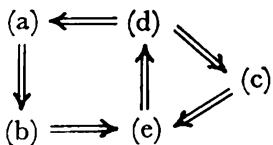
\includegraphics[keepaspectratio]{images/part001_f1dfd2f3.jpg}}

\begin{enumerate}
\def\labelenumi{(\alph{enumi})}
\item
  \(\Rightarrow\) (b): 我们知道有限生成投射模是有限表示的（第 I 章 §2 第 8 节引理 8 (iii)）；若 P 是投射 A-模，则 \(P_{m} = P \otimes_{A} A_{m}\) 是投射 \(A_{m}\) -模（《代数》第 II 章 §5 第 1 节命题 4 的推论）；最后，由于 \(A_{m}\) 是局部环，每个有限表示的投射 \(A_{m}\) -模都是自由的（§3 第 2 节命题 5 的推论）。
\item
  \(\Rightarrow\) (e): 这由第 1 节命题 2 的推论得出。
\item
  \(\Rightarrow\) (e): 设 \(m\) 是 \(A\) 的一个极大理想；记 \(r_m = n\)，并设 \((x_i)_{1 \leqslant i \leqslant n}\) 是 \(P_m\) 的一个基。我们可以假设诸 \(x_i\) 是元素 \(p_i \in P\)（\(1 \leqslant i \leqslant n\)）的典范像（至多相差 \(A_m\) 的一个可逆元的乘法）。设 \((e_i)_{1 \leqslant i \leqslant n}\) 是 \(A^n\) 的典范基，\(u: A^n \to P\) 是使 \(u(e_i) = p_i\)（对 \(1 \leqslant i \leqslant n\)）成立的同态。由于 \(P\) 是有限生成的，由第 1 节命题 2，存在 \(f \in A - m\) 使 \(u_f\) 是满射。我们得出 \(u_{fg}\) 对一切 \(g \in A - m\) 也是满射，且按假设存在 \(g \in A - m\) 使 \(r_p = n\) 对 \(p \in X_g\) 成立。于是把 \(f\) 换成 \(fg\)，我们可以假设 \(r_p = n\) 对一切 \(p \in X_f\) 成立。于是 \(u_p: A_p^n \to P_p\) 是满射同态，且 \(P_p\) 与 \(A_p\) 是同秩的自由 \(A_p\) -模；因而（§3 第 2 节命题 6 的推论）\(u_p\) 对一切 \(p \in X_f\) 是双射。设 \(p'\) 是 \(A_f\) 的一个素理想，\(p\) 是它在典范映射下在 \(A\) 中的逆像；若把 \((A_f^n)_{p'}\) 与 \((P_f)_{p'}\) 在典范同构下分别等同于 \(A_p^n\) 与 \(P_p\)，则 \((u_f)_{p'}\) 等同于 \(u_p\)，从而是双射。我们得出 \(u_f\) 是双射（§3 第 3 节定理 1），这就确立了 (e)。
\item
  \(\Rightarrow\) (d): 设 E 是 \(f\in A\)（使 \(\mathbf{P}_f\) 为有限生成自由 \(\mathbf{A}_f\) -模者）组成之集。假设蕴含 E 不含于 A 的任何极大理想，因而 E 生成理想 A，从而存在 E 中元素的有限族 \((f_{i})_{1 \leqslant i \leqslant n}\) 与 \(a_{i} \in \mathbf{A}\)（\(1 \leqslant i \leqslant n\)）使 \(1 = \sum_{i=1}^{n} a_{i} f_{i}\)；由此得 (d)。
\item
  \(\Rightarrow\) (c): 由第 1 节命题 3 的推论，P 是有限生成的。另一方面，对 A 的每个素理想 p，存在指标 \(i\) 使 \(\mathfrak{p} \in \mathrm{X}_{f_i}\)；若 \(\mathfrak{p}' = \mathfrak{p}_{f_i}\)，则 \(\mathrm{P}_{\mathfrak{p}} = (\mathrm{P}_{f_i})_{\mathfrak{p}'}\)（§2 第 5 节命题
\end{enumerate}

\begin{enumerate}
\def\labelenumi{\arabic{enumi})}
\setcounter{enumi}{9}
\tightlist
\item
因而按假设 \(\mathbf{P}_{\mathfrak{p}}\) 是自由的且与 \(\mathbf{P}_{f_i}\) 同秩，这就证明了 (c)。
\end{enumerate}

\begin{enumerate}
\def\labelenumi{(\alph{enumi})}
\setcounter{enumi}{3}
\tightlist
\item
  \(\Rightarrow\) (a): 考虑环 \(\mathbf{B} = \prod_{i\in I}\mathbf{A}_{f_i}\) 与 B-模
\end{enumerate}

\[
\mathbf {M} = \prod_ {i \in I} \mathrm{P} _ {f _ {i}} = \mathrm{P} \otimes_ {\mathbf {A}} \mathrm{B}.
\]

对每个指标 \(i\)，存在自由 \(\mathbf{A}_{f_i}\) -模 \(\mathbf{L}_i\) 使 \(\mathbf{P}_{f_i}\) 是 \(\mathbf{L}_i\) 的一个直因子，并且可以假设所有 \(\mathbf{L}_i\) 有相同的秩；则

\(L = \prod_{i \in I} L_i\) 是一个自由 B-模，M 是它的一个直因子，换言之 M 是一个有限生成投射 B-模。由于 B 是忠实平坦 A-模（第 1 节命题 3），我们得出 P 是一个有限生成投射 A-模（第 I 章 §3 第 6 节命题 12）。

推论 1. 设定理 1 陈述中的等价性质成立。设 \(m\) 是整数 \(>0\)，使得对 \((x_{i})_{1\leqslant i\leqslant m}\)（\(\mathbf{P}\) 的元素的族）的每一个，存在 \((a_{i})_{1\leqslant i\leqslant m}\)（\(\mathbf{A}\) 的元素的族），它们不全是零因子且使 \(\sum_{i=1}^{m} a_i x_i = 0\)。则对一切 \(p \in \operatorname{Spec}(A)\)，\(r_p \leqslant m\)。

设 \(p\) 是 \(A\) 的一个素理想；记 \(r = r_p\)，并设 \((y_j)_{1 \leqslant j \leqslant r}\) 是自由 \(\mathbf{A}_{p}\) -模 \(\mathbf{P}_{p}\) 的一个基。存在元素 \(x_j\)（\(1 \leqslant j \leqslant r\)，属于 \(\mathbf{P}\)）与 \(s \in A - p\) 使 \(y_j = x_j / s\) 对一切 \(j\) 成立。于是对每个元素族 \((a_j)_{1 \leqslant j \leqslant r}\)（\(A\) 的），若满足 \(\sum_{j=1}^{r} a_j x_j = 0\)，则 \(\sum_{j=1}^{r} (a_j / 1) y_j = 0\)（在 \(P_p\) 中），从而 \(a_j / 1 = 0\) 对 \(1 \leqslant j \leqslant r\) 成立。由于 \(A - p\) 不包含 0，这表明诸 \(a_j\) 都是 \(A\) 中的零因子（\(\S 2\) 第 1 节注 3），因而必然 \(r \leqslant m\)。

推论 2. 每个有限表示的平坦模都是投射模.\par

若 P 是一个有限表示的平坦 A-模而 m 是 A 的一个极大理想，则 \(A_{m}\) -模 \(P_{m}\) 是平坦的（§3 第 4 节命题 13）且有限表示的（§2 第 4 节），从而是自由的（§3 第 2 节命题 5 的推论 2），于是定理 1 的条件 (b) 成立。

注

\begin{enumerate}
\def\labelenumi{(\arabic{enumi})}
\item
  存在非投射的有限生成平坦模（习题 7）。
\item
  定理 1 的推论 2 可推广到非交换环上的模（第 I 章 §2 习题 15）。
\end{enumerate}
